\documentclass[runningheads,a4paper]{llncs}

\usepackage{azalea}
\setcounter{tocdepth}{3}

\urldef{\emails}\path|{azalea, j.villard, pg}@doc.ic.ac.uk|    
%\newcommand{\keywords}[1]{\par\addvspace\baselineskip
%\noindent\keywordname\enspace\ignorespaces#1}

\begin{document}
%
%\title{CoLoSL: \underline{Co}ncurrent \underline{Lo}cal \underline{S}ubjective \underline{L}ogic}
\title{CoLoSL: Concurrent Local Subjective Logic}
\author{Azalea Raad\and Jules Villard\and Philippa Gardner}
\institute{Imperial College London\\
\emails}

\maketitle

\begin{abstract}
A key difficulty in verifying shared-memory concurrent programs is
reasoning compositionally about each thread in isolation. Existing
verification techniques for fine-grained concurrency require 
reasoning about static global shared resource, impeding compositionality.  This
paper introduces the program logic of \colosl, where each thread is
verified with respect to its subjective view of the global
shared state.
This subjective view  just describes  that part of the global shared resource accessed by the
thread. Subjective views may arbitrarily overlap with each other, and
expand and contract depending on the resource required by the thread.
This flexibility provides truly compositional proofs for shared-memory
concurrency, which we demonstrate on a range of examples including a
concurrent computation of a spanning tree of a graph.
\end{abstract}

\allowdisplaybreaks
%\input Sections/Introduction/introduction.tex
%\input Sections/Intuition/intuition.tex
\input Sections/Model/model2.tex
%\input Sections/Assertions/assertions.tex
%\input Sections/Logic/logic.tex
%\input Sections/Semantics/semantics.tex
%\input Sections/Examples/examples.tex
\bibliographystyle{plain}
\bibliography{biblio}
\appendix{
\clearpage
\section{Existential Promotion}\label{sec:exist-promotion}
\begin{definition}[Existential promotion]
Given an assertion $P \in \Assertions$, the \emph{existential promotion} function, $\promote{.}: \Assertions \rightarrow \LAssertions$, is defined as follows:
%
\begin{mathpar}
	\promote{P} \eqdef \exists{\bar{x}^{\in S}}.\; P'
	
	\text{where } (S, P') = \ep{P}
\end{mathpar}
%
%
with the auxiliary function $\ep{.}: \Assertions \rightarrow (\pset{\textsf{LVar}} \times \Assertions)$ defined inductively over the structure of assertions as follows where $\odot \in \{\land, \lor, *, \sepish\}$.
We assume that the bound logical variables of $P$ are pairwise distinct; and that the bound variables of $P$ in $\shared{P}{I}$ do not appear free in $I$\footnote{Note that it is always possible to achieve these stipulations by renaming the bound variables in a capture-avoiding manner.}.
In what follows, $\ep{P} = (S_1, P')$ and $\ep{Q} = (S_2, Q')$ where applicable.
%
\begin{mathpar}
	\ep{A} \!\!\eqdef\! (\emptyset, A) 
	
	\ep{\shared{P}{I}} \!\!\eqdef\!  (S_1, \shared{P'}{I})
	
	\ep{P \odot Q} \!\!\eqdef\! \left(S_1 \uplus S_2, P' \odot Q' \right)

	\ep{\exsts{x}P} \!\!\eqdef\! \left({x} \uplus S_1, P'\right)
\end{mathpar}
%
\end{definition}
%
%
\begin{lemma}
Given any assertion $P \in \Assertions$, the following is valid.
%
\[
	P <=> \promote{P}
\]
%
\begin{proof}
The proof is by induction over the structure of \colosl assertions and follows from their semantics. The full proof is provided in~\cite{colosl-tr14}.
\end{proof}
\end{lemma}
\section{Overlapping Conjunction Judgements}\label{sec:sepish-judgements}
\todo
\section{Intersection Judgements}\label{sec:intersection-judgements}
%
\fig~\ref{fig:intersection-rules} presents a number of judgements for establishing that two assertions do not intersect.
%
\begin{figure}[h!]
\hrule\vspace{5pt}
\begin{mathpar}
	\infer{
		\separate{\emp}{\lass{p}}
	}
	{}
		
	\infer{
		\separate{\m{false}}{\lass{p}}
	}
	{}
	
	\infer{
		\separate{[y]}{\cell{x}{v}}
	}
	{}	

	\infer{
		\separate{[x]}{[y]}
	}
	{
		x \not= y
	}
			
	\infer{
		\separate{\cell{x}{v}}{\cell{x}{v'}}
	}
	{
		v \not= v'
	}
		
	\infer{
		\separate{\cell{x}{v}}{\cell{y}{v'}}
	}
	{
		x \not= y
	}
	
	\infer{
		\separate{(\lass{p} \septraction \lass{q})}{\lass{r}}
	}
	{
		\separate{\lass{q}}{\lass{r}}
	}
	
	\infer={
		\separate{\lass{p}}{\lass{q}}
	}
	{
		\separate{\lass{q}}{\lass{p}}
	}
	
%	[\odot \in \{*, \sepish, \land, \lor\}]
	\infer{
		\separate{(\lass{p} \odot \lass{q})}{r}
	}
	{	
		\separate{\lass{p}}{\lass{r}}
		&
		\separate{\lass{q}}{\lass{r}}
	}
	
	\infer={
		\separate{(\exsts{x} \lass{p})}{r}		
	}
	{
		\separate{(\lass{p}[v/x])}{r}
		&
		\text{for }v \in \set{Val}
	}
%
%	
\end{mathpar}
\hrule
\caption{Intersection judgements where $\odot \in \{\lor, *, ** \}$ .}
\label{fig:intersection-rules}
\end{figure}
%
%\clearpage\section{Set Module}\label{sec:set-example}
In this section we consider a concurrent set module as described in~\cite{cap-ecoop10}. We first produce the set specification in \colosl and show how to reason about its operations and verify them with respect to their specification. We then compare the \colosl specification of the set module against its specification in Concurrent Abstract Predicates (CAP) described in~\cite{cap-ecoop10}. We demonstrate that our \colosl\ reasoning considerably improves on CAP by producing a \emph{more concise} specification and allowing for \emph{more local} reasoning. 

\subsection*{\colosl Specification}
We implement a set as a sorted singly-linked list with no duplicate elements (since it represents a set) and one lock per node as described in~\cite{cap-ecoop10}. Our set module provides three operations: \li{contains(h, $v$)}, \li{add(h, $v$)} and \li{remove(h, $v$)}.
As the name suggests, the \li{contains(h, $v$)} function checks whether value $v$ is contained in the set at \li{h}; the \li{add(h, $v$)} and \command{remove(h, $v$)} functions add/remove value $v$ to/from the list, respectively.

\fig~\ref{fig:set-contains}-\ref{fig:set-locate} illustrate a possible implementation of the set operations. All three operations proceed by traversing the sorted list from the head address and locating the first node in the list holding a value $v'$ greater than or equal to $v$ (through the \li{locate} procedure). The algorithm for locating such a node begins by locking the head node; it then moves down the list by hand-over-hand locking whereby first the node following the one currently held is locked and subsequently the previously locked node is released. No thread can access a node locked by another thread or traverse past it. As such, no thread can overtake an other thread in accessing the list. 
%%
%


%
%%
%%%
%%\[
%%\begin{array}{@{} r @{\hspace*{3pt}} c @{\hspace*{3pt}} l @{}}
%%	\left\{ \inSet{\var{h}}{\var{v}} \right\} & \command{contains(h,v)} & \left\{ \inSet{\var{h}}{\var{v}} * \var{ret} = 1 \right\} \\
%%	
%%	\left\{ \outSet{\var{h}}{\var{v}} \right\} & \command{contains(h,v)} & \left\{ \outSet{\var{h}}{\var{v}} * \var{ret} = 0 \right\} \\
%%	
%%	\left\{ \inSet{\var{h}}{\var{v}} \lor \outSet{\var{h}}{\var{v}}  \right\} & \command{add(h,v)} & \left\{ \inSet{\var{h}}{\var{v}} \right\}\\ 
%%	
%%	\left\{ \inSet{\var{h}}{\var{v}} \lor \outSet{\var{h}}{\var{v}}  \right\} & \command{remove(h,v)} & \left\{ \outSet{\var{h}}{\var{v}} \right\} 
%%\end{array}
%%\]
%%%


\fig\ref{fig:coloslSetExample} shows a specification of the set module in \colosl\ similar to that of Concurrent Abstract Predicates (CAP) defined in \cite{cap-ecoop10}. 
In what follows we first give a description of the predicates of \fig\ref{fig:coloslSetExample} and subsequently contrast our specification with that of CAP.
%
%
\begin{figure}
\hrule
\[
\begin{array}{@{} l @{}}
	\begin{array}{r @{\hspace{3pt}} l}
		\inSet{h}{v} \eqdef &\exsts{\pi} \isLock{h}{\pi} *  \valueC{h}{v} * \inList{h}{v}\\	
		\outSet{h}{v} \eqdef & \exsts{\pi} \isLock{h}{\pi} * \valueC{h}{v} * \outList{h}{v} \vspace{7pt}\\
		
		\sortedList{\in}{h}{v} \eqdef & \exsts{L} \sorted{L} \land v  \in L \land \lsg{h}{\li{null}}{-\infty:: L ++ \{\infty\} }{h}\\	
		\sortedList{\not\in}{h}{v} \eqdef & \exsts{L} \sorted{L} \land v  \not\in L \land \lsg{h}{\li{null}}{-\infty:: L ++ \{\infty\} }{h} \vspace{7pt}\\
		
		\lsg{x}{z}{L}{h} \eqdef & (L = [] \land x = z \land \emp) \lor \\
		& \exsts{y, v, L'} L = v::L' \land \shared{\node{x}{v}{y}}{I(h, x)} * \lsg{y}{z}{L'}{h} \vspace{7pt}\\
		
		\node{x}{v}{y} \eqdef & \unlockedNode{x}{v}{y} \lor \lockedNode{x}{v}{y}\\
		\unlockedNode{x}{v}{y}  \eqdef & \link{x}{y} * \val{x}{v}{y}\\
		\lockedNode{x}{v}{y} \eqdef  & \locked{x} * \val{x}{v}{y} \vspace{7pt}\\
		
		\link{x}{y} \eqdef & \cell{x.next}{y} * \isLock{y}{1} * \modC{x}\\
		\val{x}{v}{y} \eqdef &  \cell{x.value}{v} * \nextC{x}{y}	\\
		
		\isLock{x}{\pi} \eqdef & \lockC{x}[\pi] * \shared{\cell{x.lock}{0} * \unlockC{x} \lor \cell{x.lock}{1}}{L(x)}\\
		\locked{x} \eqdef  & \unlockC{x} * \shared{\cell{x.lock}{1}}{L(x)}
	\end{array}	\vspace{10pt}\\
	
	
	\quad L(x) \eqdef 
	\left\{
	\begin{array}{@{} r @{\hspace{2pt}}  l @{}}
		\color{darkgreen}{\lockT{x}[-]} : &  \color{blue}{\left\{ \cell{x.lock}{0} * \unlockC{x}  \swap \cell{x.lock}{1} \right\} }\\
		\color{darkgreen}{\unlockT{x}} : &  \color{blue}{ \left\{ \cell{x.lock}{1} \swap \cell{x.lock}{0} * \unlockC{x} \right\} }\\
		\color{darkgreen}{\lockT{x} * \unlockT{x}}:  &  \color{blue}{ \left\{ \cell{x.lock}{1} \swap \lockT{x}[1] * \unlockT{x}[1] \right\} }
	\end{array}
	\right\} \vspace{10pt}\\
	

	I(h, x) \eqdef \\
	\quad
	\left\{
	\begin{array}{@{} r @ {\hspace*{2pt}}l @{}}
%%		\text{//Locking}\hspace*{1.4cm}&\\
%		\color{darkgreen}{true} : & \color{blue}{\left\{\exsts{v, y} \unlockedNode{x}{v}{y} \swap \lockedNode{x}{v}{y} \right\}}\vspace{5pt}\\
%%		\color{darkgreen}{\modT{x} } : & \color{blue}{\left\{\exsts{v, y} \lockedNode{x}{v}{y} \swap \unlockedNode{x}{v}{y} \right\}} \vspace{5pt}\\
%		
		\color{darkgreen}{true} : 
		& \color{blue}
		\left\{
		\begin{array}{@{} r @{\hspace{2pt}} l @{\hspace{3pt}} l @{\hspace{3pt}} l @{}}
			\exsts{v, y} & \unlockedNode{x}{v}{y} & \swap & \lockedNode{x}{v}{y} \vspace{5pt}\\
			\exsts{v, y} & \lockedNode{x}{v}{y} & \swap & \unlockedNode{x}{v}{y}
		\end{array}		
		\right\}		\vspace{5pt}\\
		
		
		
		\color{darkgreen}{\modT{x} * \valueT{h}{v}:} & \\		
		&\hspace{-2.7cm}   
		\color{blue}{\left\{
		\begin{array}{@{} l @{\hspace{5pt}} l @{}}
			\exsts{v',y, z} & \lockedNode{x}{v'}{y} * \lockedNode{y}{v}{z}\\
			& \quad \swap \lockedNode{x}{v'}{z} * \lockedNode{y}{v}{z}\\
			
			\exsts{v', w, y} & v' < v /| \lockedNode{w}{v'}{y} * \lockedNode{x}{v}{y}\\
			& \quad \swap \lockedNode{w}{v'}{y}\\
			
			\exsts{v_1,\! v_2,\! y,\! z,\! w} & v_1 < v < v_2 \land \lockedNode{x}{v_1}{y} * \val{w}{v}{y} * \val{y}{v_2}{z} \\
	  	& \quad \swap \lockedNode{x}{v_1}{w} * \val{w}{v}{y} *  \val{y}{v_2}{z}		
		\end{array}
		\right\}
		}

		
	\end{array}
	\right\}


	
%	I(h, a) \eqdef 
%	\left\{
%	\begin{array}{@{} r @ {\hspace*{2pt}}l @{} }
%%		\text{//Locking}\hspace*{1.4cm}&\\
%		\lockT{a}: &\left\{ \exsts{v, b} \unlockedNode{a}{v}{b} \swap \lockedNode{a}{v}{b}\right\} \vspace{5pt}\\
%		
%%		\text{//Unlocking}\hspace*{1.1cm}&\\
%		\unlockT{a}: & \left\{ \exsts{v, b} \lockedNode{a}{v}{b} \swap \unlockedNode{a}{v}{b}\right\} \vspace{5pt}\\ 
%		
%%		\text{//Deletion of } v \hspace*{0.8cm}&\\
%		\unlockT{a} * \valueT{h}{v}: &
%		\left\{
%		\begin{array}{@{} l @{\hspace{5pt}} l @{}}
%			\exsts{v_0, b, c} & \lockedNode{a}{v_0}{b} * \lockedNode{b}{v}{c} \\
%			& \quad \swap \lockedNode{a}{v_0}{c} * \lockedNode{b}{v}{c} \\
%			\exsts{v_0, b, c} & \lockedNode{b}{v_0}{c} * \lockedNode{a}{v}{c} \\
%			& \quad \swap \lockedNode{b}{v_0}{c} 
%			
%		\end{array}
%		\right\} \vspace{5pt}\\ 
%
%		
%%		\text{//Insertion of } v \hspace*{0.7cm}&\\
%		\unlockT{a} * \valueT{h}{v}: &\\
%		&\hspace{-3cm}
%		\left\{
%		\begin{array}{@{} l @{\hspace{4pt}} l @{}}
%			\exsts{v_1, v_2, c, d} & v_1 < v < v_2 \land \lockedNode{a}{v_1}{c} * \lockedNode{c}{v_2}{d} \\
%			& \quad \swap \lockedNode{a}{v_1}{b} * \node{b}{v}{c} *  \lockedNode{c}{v_1}{d}\\
%			 
%			\exsts{v_1, v_2, c, d} & v_1 < v < v_2 \land \lockedNode{a}{v_1}{c} * \unlockedNode{c}{v_2}{d} \\
%			& \quad \swap \lockedNode{a}{v_1}{b} * \node{b}{v}{c} *  \unlockedNode{c}{v_1}{d}
%						
%		\end{array}
%		\right\}\\ 
%		
%	\end{array}
%	\right\}
\end{array}
\]
%
\hrule
\caption{\colosl\ specification of the concurrent set module.}
\label{fig:coloslSetExample}
\end{figure}
%
%

Since \colosl is parametric in the separation algebra of capabilities and their assertions, we instantiate it with a \emph{fractional heap} to represent the separation algebra of capabilities and write heap-like assertions of the form $\setCap{a}[\pi][b]$ to denote capability $a$ with permission $\pi$. Moreover, our capabilities are \emph{stateful} in that they can capture some additional information ($b$). As we demonstrate below, this leads to conciser specifications. For readability we write $\setCap{a}[][b]$ for $\setCap{a}[1][b]$, $\setCap{a}[\pi]$ for $\exsts{b}\setCap{a}[\pi][b]$ and $\setCap{a}$ for $\exsts{b}\setCap{a}[1][b]$.

%\noindent\textbf{\textsf{isLock}($a, \pi$) / \textsf{locked}($a$)} \hspace{0.3cm} 
\paragraph{\textbf{\textsf{isLock(}\textit{x}, $\pi$\textsf{)} / \textsf{locked(}\textit{x}\textsf{)}}} 
Every node in the singly-linked list is protected by a lock that is to be acquired prior to its modification. The $\isLock{x}{\pi}$ predicate is similar to that in \cite{cap-ecoop10} and states that the lock at address $x$ can be acquired with permission $\pi \in (0, 1]$. Multiple threads may attempt to acquire the lock at once and thus we use the $\pi$ argument to reflect this sharing where $1$ denotes exclusive right to acquisition while $\pi \in (0, 1)$ accounts for sharing of the lock between multiple threads. The $\isLock{x}{\pi}$ predicate asserts that the thread's local state contains the capability $\lockT{x}[\pi]$ to acquire the lock and that the lock resides in the shared state where at any one point either the lock is unlocked ($\cell{x.lock}{0}$) and the shared state contains the capability to unlock it ($\unlockT{x}$); or it is locked ($\cell{x.lock}{1}$) and the unlocking capability has been claimed by the locking thread. 

The $\locked{x}$ predicate asserts that the thread's local state contains the exclusive capability to unlock the lock ($[\unlockT{x}]$); and that the $x$ is in the locked state ($\cell{x.lock}{1}$). 

\paragraph{\textbf{\textit{L}\textsf{(}\textit{x}\textsf{)}}} denotes the interference associated with the lock on node at address $x$. When a thread holds a non-zero locking capability on node $x$ ($\lockC{x}[-]$), it can change the lock state from unlocked (0) to locked (1) and claim the exclusive unlocking capability in doing so ($\unlockC{x}$). 
Similarly, a thread holding the full unlocking capability on $x$ ($\unlockC{x}$) can change the lock state from locked to unlocked and return the full unlocking capability to the shared state. 
When removing a value $v$ from the set, the node containing the value $v$ must be removed from the shared state and disposed of. However, recall that \colosl does not have an explicit mechanism for unsharing resources modelling a dual behaviour to that of the \extendRule principle. Instead, resources can be unshared through actions explicitly specified as part of their associated interference. This is the case in the last component of $L(x)$; it is concerned with \emph{unsharing} of node $x$'s lock and making it a local resource. It states that when a thread holds full permission on both locking and unlocking capabilities of $x$, it can claim its lock in exchange for the capabilities. 

\paragraph{\textbf{\textsf{in(}\textit{h}, \textit{v}\textsf{)} / \textsf{out(}\textit{h}, \textit{v}\textsf{)}}}
The $\inSet{h}{v}$ predicate states that the set at head address $h$ contains value $v$ and captures exclusive right to alter the set with respect to $v$ by changing whether $v$ belongs to it. It asserts that the thread owns some capability ($\pi$) to acquire the lock associated with head address ($\isLock{h}{\pi}$) and that the thread owns the exclusive capability to alter the set with respect to value $v$ ($\valueC{h}{v}$) should it own the capability to modify the address at which value $v$ is stored (\textit{cf.} the description of $\unlockedNode{x}{v}{y}$ predicate). The underlying singly-inked list is captured by the $\inList{h}{v}$ predicate. 
The $\inList{h}{v}$ predicate uses an auxiliary carrier sorted list $L$ (such that $v \in L$) to capture the contents of the singly-linked list via the $\textsf{lsg}$ predicate. For simpler implementation, we extend $L$ with two sentinel values $-\infty$ and $\infty$, one at each end to avoid corner cases such as removing the first/last element of the list. The $\outSet{h}{v}$ predicate is analogous to $\inSet{h}{v}$ and corresponds to the case where the set does not contain $v$.

\paragraph{\textbf{\textsf{lsg(}\textit{x}, \textit{z}, \textit{L}, \textit{h}\textsf{)}}} 
This predicate is defined inductively and describes a \emph{segment} of the list at $h$ that starts at address $x$ and extends upto (but not including) address $z$ and contains the elements in the mathematical list $L$. When $L$ is empty, it corresponds to a void segment and yields no resources (\emp); otherwise, it is defined as the composition of the first node of the segment at address $x$, $\shared{\node{x}{v}{y}}{I(h, x)}$, and the tail of the list segment ($\lsg{y}{z}{L'}{h}$). The $\node{x}{v}{y}$ predicate describes a node at address $x$ with value $v$ and successor $y$ and can be either unlocked ($\unlockedNode{x}{v}{y}$) or locked ($\lockedNode{x}{v}{y}$).

\paragraph{\textbf{\textsf{U(}\textit{x}, \textit{v}, \textit{y}\textsf{)} / \textsf{L(}\textit{x}, \textit{v}, \textit{y}\textsf{)}}}
The $\unlockedNode{x}{v}{y}$ predicate states that the node at address $x$ is unlocked, it contains value $v$ and comes before the node at address $y$. The statement of the $\lockedNode{x}{v}{y}$ predicate is analogous and describes the node when locked.
%In both locked and unlocked states, the shared state contains the lock field ($\cell{a}{0}$ or $\cell{a}{1}$), the value field ($\cell{a+1}{v}$) and the capability that records the current successor of the node $\nextC{a}{b}$.
%When a node is in the unlocked state, the shared state contains the next pointer of the node ($\cell{a+2}{b}$), as well as the capability to unlock the node ($[\unlockT{a}]$).
%% A thread can alter the set at $h$ with respect to the node at $a$ with value $v$ only when it holds both the value capability $\valueC{h}{v}$ and the modification capability $\modC{a}$ in its local state. 
%Recall that when traversing the list by hand-over-hand locking, no thread can overtake an other in traversing the list. Consequently, a node can only be locked by a thread that has already acquired the lock associated with the previous node. 
%As such, when the node $a$ is in the unlocked state, the exclusive capability to lock the successor node at address $b$ ($[\lockT{b}]$) also lies in the shared state.
%% 
%
%When a thread successfully locks the node at $a$ it claims the next pointer, the unlocking capability and the locking capability pertaining to its successors. ($\cell{a.next}{b} * [\unlockT{a}] * [\lockT{b}]$) and moves them into its local state.
%\\
%
%A thread can alter the set at $h$ with respect to the node at address $x$ with value $v$, only when it holds both the value capability $\valueC{h}{v}$ and the modification capability $\modC{x}$ in its local state. When the node is in the unlocked state, no thread can modify it and thus the modification capability $\modC{x}$ as well as the next pointer of the node ($\cell{x.next}{y}$) lie in the shared state. 
A thread may modify the next pointer of node at address $x$, only when it holds the modification capability $\modC{x}$ in its local state. When the node is in the unlocked state, no thread can modify it and thus the modification capability $\modC{x}$ as well as the next pointer of the node ($\cell{x.next}{y}$) lie in the shared state. 
%
Recall that when traversing the list by hand-over-hand locking, no thread can overtake an other in traversing the list. Consequently, a node can only be locked by a thread that has already acquired the lock associated with the previous node. Therefore, when the node $x$ is in the unlocked state, the exclusive capability to lock its successor at address $y$ ($\isLock{y}{1}$) also lies in the shared state.
%
When a thread successfully locks the node at $x$ (and is hence in possession of the $\locked{x}$ resource), it can then claim the next pointer, the modification capability and the locking capability pertaining to its successors (captured by $\link{x}{y}$), and move them into its local state. In return, it transfers the $\locked{x}$ resource to the shared state as evidence that it is indeed the locking thread.

In both locked and unlocked states, the shared state contains the value field ($\cell{x.value}{v}$) and the ``successor'' capability $\nextC{x}{y}$. This capability is used to track the current successor of $x$ even when the node is locked and its next pointer has been claimed by the locking thread. 

\paragraph{\textbf{\textit{I}\textsf{(}\textit{h}, \textit{x}\textsf{)}}} As discussed above, given a node at address $x$ with successor $y$, any thread in possession of the $\locked{x}$ resource may change its state from unlocked ($\unlockedNode{x}{v}{y}$) to locked ($\lockedNode{x}{v}{y}$) and claim the $\link{x}{y}$ resource in exchange for $\locked{x}$. This is captured by the first action associated with the $\m{true}$ assertion; that is, no additional capability is required for performing this action and holding the $\locked{x}$ resource locally is sufficient for performing the action. Conversely, as described by the second action of $\m{true}$, a thread in possession of the $\link{x}{y}$ resource may change its state from locked ($\lockedNode{x}{v}{y}$) to unlocked ($\unlockedNode{x}{v}{y}$) and return $\link{x}{y}$ to the shared state in return for $\locked{x}$. 

Consider a node at address $y$, with value $v$, successor $z$ and predecessor $x$. A thread may remove value $v$ from the set provided that both the node and its predecessor are locked by the thread; and the thread holds the value capability $\valueC{h}{v}$ as well as the update capabilities pertaining to both the node itself ($\modC{x}$) and its predecessor node ($\modC{y}$). This is captured by the first two actions associated with $\modC{x} * \valueC{h}{v}$ in $I(h, x)$. First, the next pointer of $x$ is redirected to $z$ (the first action of $\modC{x} * \valueC{h}{v}$); and then node $y$ is removed from the shared state (the second action of $\modC{y} * \valueC{h}{v}$).
Similarly, for a thread to insert the value $v$ in between node $x$ and node $y$, the predecessor node $x$ must be locked; and the thread should hold the value capability $\valueC{h}{v}$ as well as the update capability on $x$. This is reflected in the last action of $\modC{x} * \valueC{h}{v}$.

\subsection*{Reasoning about Set Operations}
%
\fig~\ref{fig:set-contains}-\ref{fig:set-locate} illustrate the implementation of the set operations along with an outline of the reasoning steps involved in establishing their correctness against their \colosl specification. In what follows, we give an account of reasoning about the set \li{add} operation as outlined in \fig~\ref{fig:set-add}; we demonstrate that given a set at address \li{h}, where value $v$ may or may not be present in the set, after a call to the \li{add(h, $v$)} operation the set will contain the value $v$. That is, the \li{add(h, $v$)} operation satisfies the following specification.
%
\[
\begin{array}{c}
	\color{blue}\left\{ \inSet{\li h}{v} \lor \outSet{\li h}{v} \right\}\\
	\li{add(h, $v$)}\\
	\color{blue}\left\{ \inSet{\li h}{v} \right\}
\end{array}
\]
%
The implementation of \li{add} proceeds by locating the index at which the new node is to be inserted through a call to the \li{locate(h, $v$)} operation. The \li{locate(h, $v$)} call traverses the list by hand-over-hand locking until it locates the addresses of node $p$ with value $v_p$ and node $c$ with value $v_c$ such that $v_p < v \leq v_c$. It then locks $p$ and claims its next pointer ($\link{\li p}{\li c}$) as allowed by $L(\li{p})$. Note that since the list contains the sentinel values $-\infty$ and $+\infty$ at either end, for any given value $v'$ the locate operation always finds $v_1$ and $v_2$ such that $v_1 < v' \leq v_2$. 
%The following depicts the state of the set upon return from the \li{(p, c):= locate(h, $v$)} call.
%%
%\[
%	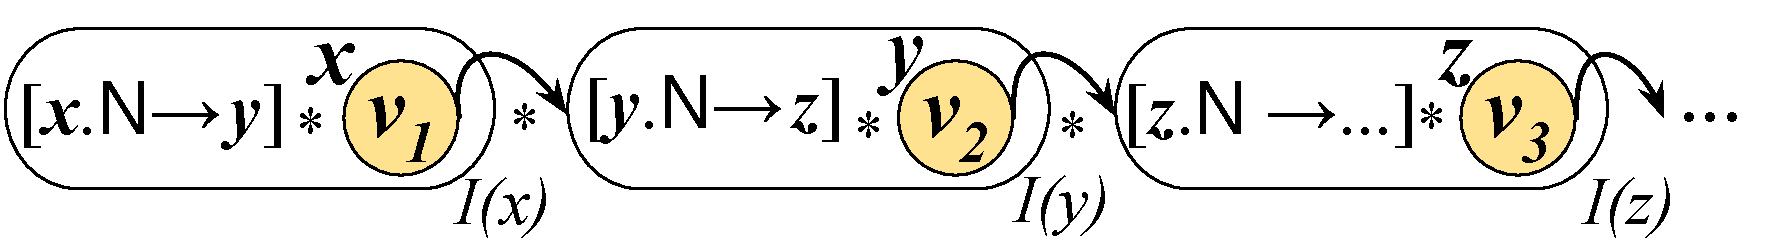
\includegraphics[scale=0.24]{Sections/Examples/Images/coloslSet.pdf}
%\]
%%{\centering 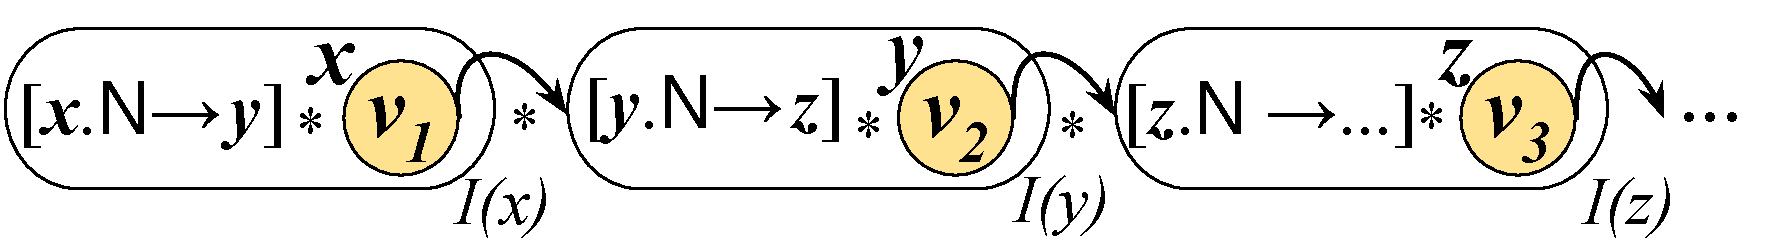
\includegraphics[scale=0.24]{Sections/Examples/Images/coloslSet.pdf}\\}
%%
If \li{c.value = $v$} and consequently the set contains value $v$, node $p$ is unlocked and the operating thread simply returns. On the other hand if $v_c > v$,  
%\noindent Since \colosl\ allows for \emph{dynamic} extension of the shared state, we do not need to account for capabilities associated with \emph{all} possible addresses. Instead, fresh capabilities are generated dynamically as needed. We demonstrate this by giving an outline of reasoning about the \li{add(}$v'$\li{)} method. 
%
a new node $z$ with value $v$ and successor $c$ is allocated and the shared state is extended by the resources associated with the new node $z$ as follows. First, the shared state is extended by $z$'s lock and in doing so the locking and unlocking capabilities pertaining to $z$ are generated on the fly. That is the $\cell{\li{z.lock}}{0}$ predicate is replaced by $\isLock{z}{1}$ as shown in the following derivation.
%
\small
\begin{align*}
	&\color{blue}
	\left\{
 	\begin{array}{@{} l @{}}
	 	\exsts{L_1, L_2, v_p, v_c, \pi} v_p < v < v_c \land \sorted{L_1 ++ \{v_p\} ++ v_c :: L_2}  \land\\
	 	\isLock{\!\li h}{\pi} * \valueT{\!\li h}{v}  		 	
		* \lsg{\!\li h}{\!\li p}{L_1}{\!\li h} \\		
	 	* \shared{\lockedNode{\!\li p}{v_p}{\!\li c}}{I(\!\li p)} 
	 	* \link{\!\li p}{\!\li c}
	 	* \lsg{\!\li c}{\li{null}}{v_c ::L_2}{\!\li h} 	
 	\end{array}
 	\right\}\\
%
%
	\stackrel{\text{(frame off)}}{}
	& \quad\color{blue}
	\left\{ \emp \right\}\\
%
%
	\stackrel{\text{alloc+assign}}{\semimplies}
	& \quad \color{blue}
	\left\{
		\cell{\!\li{z.value}}{v}	
		* \cell{\!\li{z.next}}{\!\li c}
		* \cell{\!\li{z.lock}}{0}
	\right\}\\
%
%
	\stackrel{\extendRule}{\semimplies}
	& \quad \color{blue}
	\left\{
		\cell{\!\li{z.value}}{v}	
		* \cell{\!\li{z.next}}{\li c}
		* \lockT{\!\li z} 
		* \shared{\cell{\!\li{z.lock}}{0} * \unlockT{\!\li z}}{L(\!\li z)}
	\right\}\\
%
%	
	%
%
	\stackrel{\textsf{isLock} \text{ def.}}{}
	& \quad \color{blue}
	\left\{
		\cell{\!\li{z.value}}{v}	
		* \cell{\!\li{z.next}}{\!\li c}
		* \isLock{\!\li z} {1}
	\right\}\\
%
%	
	\stackrel{\text{(frame on)}}{} 
	&\color{blue}
	\left\{
 	\begin{array}{@{} l @{}}
	 	\exsts{L_1, L_2, v_p, v_c, \pi} v_p < v < v_c \land \sorted{L_1 ++ \{v_p\} ++ v_c :: L_2}  \land\\
	 	\isLock{\!\li h}{\pi} * \valueT{\!\li h}{v}  		 	
		* \lsg{\!\li h}{\!\li p}{L_1}{\!\li h} \\		
	 	* \shared{\lockedNode{\!\li p}{v_p}{\!\li c}}{I(\!\li p)} 
	 	* \link{\!\li p}{\!\li c}
	 	* \lsg{\!\li c}{\li{null}}{v_c ::L_2}{\!\li h} 	\\
	 	* \cell{\!\li{z.value}}{v}	
		* \cell{\!\li{z.next}}{\!\li c}
	 	* \isLock{\!\li z} {1}
 	\end{array}
 	\right\}
%
%
\end{align*}\normalsize
%\[
%	\cell{\li{z.lock}}{0} \semimplies \lockT{\li z} * \shared{\cell{\li{z.lock}}{0} * \unlockT{\li z}}{L(\li z)} \implies \isLock{\li z}{1}
%\]
%
The shared state is then extended with the remaining resources of node $\li z$ and the relevant capabilities are also generated; subsequently, the subjective views of nodes $p$, $z$ and $c$ are combined through an application of the \mergeRule principle as demonstrated by the following derivation. 
%
\small
\begin{align*}
	& 
	\color{blue} 
	\left\{
 	\begin{array}{@{} l @{}}
	 	\exsts{L_1, L_2, v_p, v_c, \pi} v_p < v < v_c \land \sorted{L_1 ++ \{v_p\} ++ v_c :: L_2}  \land\\	 	
	 	\isLock{\!\li h}{\pi} * \valueT{\!\li h}{v}  		 	
		* \lsg{\!\li h}{\!\li p}{L_1}{\!\li h} \\		
	 	* \shared{\lockedNode{\!\li p}{v_p}{\!\li c}}{I(\!\li p)} 
	 	* \link{\!\li p}{\!\li c}
	 	* \lsg{\!\li c}{\li{null}}{v_c ::L_2}{\!\li h}\\	 	
	 	* \cell{\!\li{z.value}}{v} * \cell{\!\li{z.next}}{\!\li c} * \isLock{\li z}{1} 	
 	\end{array}
 	\right\}\\
%	 	
%	 	
	\stackrel{\text{(frame off)}}{} & 
	\quad\color{blue} 
	\left\{ 
		\link{\!\li p}{\!\li c} * \cell{\!\li{z.value}}{v} * \cell{\!\li{z.next}}{\!\li c} 
	\right\}\\
%	
%
	\stackrel{\textsf{link}\text{ def.}}{\implies} & 
	\quad\color{blue} 
	\left\{
		\cell{\!\li{p.next}}{\!\li c} * \modC{\!\li p} * \isLock{\!\li c}{1}  * \cell{\!\li{z.next}}{\!\li c} * \cell{\!\li{z.value}}{v}
	\right\}\\
%	
%
	\stackrel{\extendRule}{\semimplies} & 
	\quad\color{blue} 
	\left\{
		\cell{\!\li{p.next}}{\!\li c} * \modC{\!\li p} * 
		\shared{
			\begin{array}{@{} l @{}}
				\isLock{\!\li c}{1}  * \cell{\!\li{z.next}}{\!\li c} * \modC{\!\li z}\\
				* \cell{\!\li{z.value}}{v} * \nextC{\!\li z}{\li c}
			\end{array}
		}{I(\li z)}
	\right\}\\
%	
%	
	\stackrel{\textsf{U}\text{ def.}}{\implies} & 
	\quad\color{blue} 
	\left\{
		\cell{\!\li{p.next}}{\!\li c} * \modC{\!\li p} * 
		\shared{
			\begin{array}{@{} l @{}}
				\unlockedNode{\li z}{v}{\li c}
			\end{array}
		}{I(\li z)}
	\right\}\\
%	
%	
	\stackrel{\textsf{node}\text{ def.}}{\implies} & 
	\quad\color{blue} 
	\left\{
		\cell{\!\li{p.next}}{\!\li c} * \modC{\!\li p} * 
		\shared{
			\begin{array}{@{} l @{}}
				\node{\li z}{v}{\li c}
			\end{array}
		}{I(\li z)}
	\right\}\\
%	
%	
	\stackrel{\text{(frame on)}}{} 
	& \color{blue} 
	\left\{
 	\begin{array}{@{} l @{}}
	 	\exsts{L_1, L_2, v_p, v_c, \pi} v_p < v < v_c \land \sorted{L_1 ++ \{v_p\} ++ v_c :: L_2}  \land\\ 	
	 	\isLock{\!\li h}{\pi} * \valueT{\!\li h}{v}  		 	
		* \lsg{\!\li h}{\!\li p}{L_1}{\!\li h} \\		
	 	* \shared{\lockedNode{\!\li p}{v_p}{\!\li c}}{I(\!\li p)} 
	 	* \cell{\!\li{p.next}}{\!\li c} * \modC{\!\li p} 
	 	* \lsg{\!\li c}{\li{null}}{v_c ::L_2}{\!\li h}\\ 	
	 	* \shared{
			\begin{array}{@{} l @{}}
				\node{\li z}{v}{\li c}
			\end{array}
		}{I(\li z)}
		* \isLock{\li z}{1}
 	\end{array}
 	\right\}\\
%	
%	
	\stackrel{\textsf{lsg}\text{ def.}}{\implies} 
	& \color{blue} 
	\left\{
 	\begin{array}{@{} l @{}}
	 	\exsts{L_1, L_2, v_p, v_c, \pi, d} v_p < v < v_c \land \sorted{L_1 ++ \{v_p\} ++ v_c :: L_2}  \land\\ 	
	 	\isLock{\!\li h}{\pi} * \valueT{\!\li h}{v}  		 	
		* \lsg{\!\li h}{\!\li p}{L_1}{\!\li h} \\		
	 	* \shared{\lockedNode{\!\li p}{v_p}{\!\li c}}{I(\!\li p)} 
	 	* \cell{\!\li{p.next}}{\!\li c} * \modC{\!\li p} 
	 	* \shared{\lockedNode{\!\li c}{v_c}{\!\li d}}{I(\!\li c)} \\	 	
	 	* \lsg{\!\li d}{\li{null}}{L_2}{\!\li h}
	 	* \shared{
			\begin{array}{@{} l @{}}
				\node{\li z}{v}{\li c}
			\end{array}
		}{I(\li z)}
		* \isLock{\li z}{1}
 	\end{array}
 	\right\} 	\\
%
%	
	\stackrel{\text{\mergeRule}\times 2}{\implies} 
	& \color{blue} 
	\left\{
 	\begin{array}{@{} l @{}}
	 	\exsts{L_1, L_2, v_p, v_c, \pi, d} v_p < v < v_c \land \sorted{L_1 ++ \{v_p\} ++ v_c :: L_2}  \land\\ 	
	 	\isLock{\!\li h}{\pi} * \valueT{\!\li h}{v}  		 	
		* \lsg{\!\li h}{\!\li p}{L_1}{\!\li h} \\		
	 	* \shared{\lockedNode{\!\li p}{v_p}{\!\li c} * \node{\li z}{v}{\li c} * \lockedNode{\!\li c}{v_c}{\!\li d} * }{I(\!\li p) \cup I(\li z) \cup I(\!\li c)} \\
	 	* \cell{\!\li{p.next}}{\!\li c} * \modC{\!\li p} 
	 	* \lsg{\!\li d}{\li{null}}{L_2}{\!\li h}
		* \isLock{\li z}{1}
 	\end{array}
 	\right\} 	
%
% 
\end{align*}	
\normalsize
%
At this point, since the locking thread holds the next pointer of $p$ in its local state ($\cell{\li{p.next}}{\li c}$), it modifies it to point to the new node $z$; and through the action of $\modC{\li p} * \valueC{\li h}{v}$, the $\lockedNode{\li p}{v_p}{\li c}$ predicate is updated as $\lockedNode{\li p}{v_p}{\li z}$. Recall that the $\lockedNode{\li p}{v_p}{\li c}$ predicate states that the node at \li{p} is locked, it holds value $v_p$ and prior to locking its successor was the node at address \li{c}. As such, since the value of the new node $\li{z}$ lies between that of \li{p} and \li{c} ($v_p < v < v_c$), this action allows us to insert \li{z} in between \li{p} and \li{c} provided that \li{z} itself points to \li{c}. This is captured by the following derivation where ($\dagger$) denotes the application of the action associated with the $\modC{\li p} * \valueC{\li h}{v}$ capability in $I(\li p)$.
%That is $\shared{\lockedNode{\li p}{v_p}{\li c} * \node{\li z}{v}{\li c} * \node{\li c}{v_c}{d}}{I(\li p) \cup I(\li z) \cup I(\li c)}$ is updated as $\shared{\lockedNode{\li p}{v_p}{\li z} * \node{\li z}{v}{\li c} * \node{\li c}{v_c}{d}}{I(\li p) \cup I(\li z) \cup I(\li c)}$.
%
\small
\begin{align*}
	& \color{blue} 
	\left\{
 	\begin{array}{@{} l @{}}
	 	\exsts{L_1, L_2, v_p, v_c, \pi, d} v_p < v < v_c \land \sorted{L_1 ++ \{v_p\} ++ v_c :: L_2}  \land\\ 	
	 	\isLock{\!\li h}{\pi} * \valueT{\!\li h}{v}  		 	
		* \lsg{\!\li h}{\!\li p}{L_1}{\!\li h} \\		
	 	* \shared{\lockedNode{\!\li p}{v_p}{\!\li c} * \node{\li z}{v}{\li c} * \lockedNode{\!\li c}{v_c}{\!\li d} * }{I(\!\li p) \cup I(\li z) \cup I(\!\li c)} \\
	 	* \cell{\!\li{p.next}}{\!\li c} * \modC{\!\li p} 
	 	* \lsg{\!\li d}{\li{null}}{L_2}{\!\li h}
		* \isLock{\li z}{1}
 	\end{array}
 	\right\} 	\\
%
% 
	\stackrel{(\!\li{p.next:= z})}{\implies} 
	& \color{blue} 
	\left\{
 	\begin{array}{@{} l @{}}
	 	\exsts{L_1, L_2, v_p, v_c, \pi, d} v_p < v < v_c \land \sorted{L_1 ++ \{v_p\} ++ v_c :: L_2}  \land\\ 	
	 	\isLock{\!\li h}{\pi} * \valueT{\!\li h}{v}  		 	
		* \lsg{\!\li h}{\!\li p}{L_1}{\!\li h} \\		
	 	* \shared{\lockedNode{\!\li p}{v_p}{\!\li c} * \node{\li z}{v}{\li c} * \lockedNode{\!\li c}{v_c}{\!\li d} * }{I(\!\li p) \cup I(\li z) \cup I(\!\li c)} \\
	 	* \cell{\!\li{p.next}}{\!\li z} * \modC{\!\li p} 
	 	* \lsg{\!\li d}{\li{null}}{L_2}{\!\li h}
		* \isLock{\li z}{1}
 	\end{array}
 	\right\} 	\\
%
% 
	\stackrel{\textsf{link}\text{ def.}}{\implies} 
	& \color{blue} 
	\left\{
 	\begin{array}{@{} l @{}}
	 	\exsts{L_1, L_2, v_p, v_c, \pi, d} v_p < v < v_c \land \sorted{L_1 ++ \{v_p\} ++ v_c :: L_2}  \land\\ 	
	 	\isLock{\!\li h}{\pi} * \valueT{\!\li h}{v}  		 	
		* \lsg{\!\li h}{\!\li p}{L_1}{\!\li h} \\		
	 	* \shared{\lockedNode{\!\li p}{v_p}{\!\li c} * \node{\li z}{v}{\li c} * \lockedNode{\!\li c}{v_c}{\!\li d} * }{I(\!\li p) \cup I(\li z) \cup I(\!\li c)} 
	 	* \link{\li p}{\li z}
 	\end{array}
 	\right\} 	\\
%
% 
	\stackrel{(\dagger)}{\semimplies} 
	& \color{blue} 
	\left\{
 	\begin{array}{@{} l @{}}
	 	\exsts{L_1, L_2, v_p, v_c, \pi, d} v_p < v < v_c \land \sorted{L_1 ++ \{v_p\} ++ v_c :: L_2}  \land\\ 	
	 	\isLock{\!\li h}{\pi} * \valueT{\!\li h}{v}  		 	
		* \lsg{\!\li h}{\!\li p}{L_1}{\!\li h} \\		
	 	* \shared{\lockedNode{\!\li p}{v_p}{\!\li z} * \node{\li z}{v}{\li c} * \lockedNode{\!\li c}{v_c}{\!\li d} * }{I(\!\li p) \cup I(\li z) \cup I(\!\li c)} 
	 	* \link{\li p}{\li z}
 	\end{array}
 	\right\} 	
%
% 
\end{align*}
\normalsize
%
All that remains is to unlock the node at \li{p}; to do this, first the state of the node is changed from locked ($\lockedNode{\li{p}}{v_p}{\li{z}}$) to unlocked ($\unlockedNode{\li{p}}{v_p}{\li{z}}$) by applying the action of $\modC{\li p}$ capability. Subsequently, through several applications of \copyRule, \forgetRule and \shiftRule principles, the subjective views of \li{p}, \li{z} and \li{c} nodes are recovered as follows where ($\dagger$) denotes the application of the action associated with the $\modC{\li p}$ capability in $I(\li p)$.
%
\small
\begin{align*}
	& \color{blue} 
		\left\{
	 	\begin{array}{@{} l @{}}
		 	\exsts{L_1, L_2, v_p, v_c, \pi, d} v_p < v < v_c \land \sorted{L_1 ++ \{v_p\} ++ v_c :: L_2}  \land\\ 	
		 	\isLock{\!\li h}{\pi} * \valueT{\!\li h}{v}  		 	
			* \lsg{\!\li h}{\!\li p}{L_1}{\!\li h} \\		
		 	* \shared{\lockedNode{\!\li p}{v_p}{\!\li z} * \node{\li z}{v}{\li c} * \lockedNode{\!\li c}{v_c}{\!\li d} * }{I(\!\li p) \cup I(\li z) \cup I(\!\li c)} 
		 	* \link{\li p}{\li z}
	 	\end{array}
	 	\right\} 	\\
%
% 
	\stackrel{\text{(frame off)}}{}
	& \quad \color{blue} 
		\left\{ 
			\shared{\lockedNode{\!\li p}{v_p}{\!\li c} * \node{\!\li z}{v}{\!\li c} * \node{\!\li c}{v_c}{d}}{I(\!\li p) \cup I(\!\li z) \cup I(\!\li c)}
			* \link{\!\li p}{\!\li z}
		\right\}\\
%	
%	
	\stackrel{(\dagger)}{\semimplies}
	& \quad \color{blue} 
		\left\{
			\shared{\unlockedNode{\!\li p}{v_p}{\!\li z} * \node{\!\li z}{v}{\!\li c} * \node{\!\li c}{v_c}{d}}{I(\!\li p) \cup I(\!\li z) \cup I(\!\li c)}
			* \locked{\!\li p}
		\right\}\\
%
%	
	\stackrel{\textsf{node}\text{ def.}}{\implies} 
	& \quad \color{blue} 
		\left\{
			\shared{\node{\!\li p}{v_p}{\!\li z} * \node{\!\li z}{v}{\!\li c} * \node{\!\li c}{v_c}{d}}{I(\!\li p) \cup I(\!\li z) \cup I(\!\li c)} 
			\!\!* \locked{\!\li p}
		\right\} \vspace{7pt}\\
%
%	
	\stackrel{\copyRule \times 2}{\implies} 
	& \quad \color{blue} 
	\left\{
	\begin{array}{@{} l @{}}
		\shared{\node{\!\li p}{v_p}{\!\li z} * \node{\!\li z}{v}{\!\li c} * \node{\!\li c}{v_c}{d}}{I(\!\li p) \cup I(\!\li z) \cup I(\!\li c)}\\
		* \shared{\node{\!\li p}{v_p}{\!\li z} * \node{\!\li z}{v}{\!\li c} * \node{\!\li c}{v_c}{d}}{I(\!\li p) \cup I(\!\li z) \cup I(\!\li c)}\\
		* \shared{\node{\!\li p}{v_p}{\!\li z} * \node{\!\li z}{v}{\!\li c} * \node{\!\li c}{v_c}{d}}{I(\!\li p) \cup I(\!\li z) \cup I(\!\li c)}\\
		* \locked{\!\li p}
	\end{array}
	\right\} \vspace{7pt}\\
%	
%	
	\stackrel{\forgetRule \times 3}{\implies} 
	& \quad \color{blue} 
	\left\{
	\begin{array}{@{} l @{}}
		\shared{\node{\!\li p}{v_p}{\!\li z}}{I(\!\li p) \cup I(\!\li z) \cup I(\!\li c)}
		* \shared{\node{\!\li z}{v}{\!\li c}}{I(\!\li p) \cup I(\!\li z) \cup I(\!\li c)}\\
		* \shared{\node{\!\li c}{v_c}{d}}{I(\!\li p) \cup I(\!\li z) \cup I(\!\li c)} * \locked{\!\li p}
	\end{array}
	\right\} \vspace{7pt}\\
%	
%	
	\stackrel{\shiftRule \times 3}{\semimplies} 
	& \quad \color{blue} 
	\left\{\shared{\node{\!\li p}{v_p}{\!\li z}}{I(\!\li p)}
	\!\!* \shared{\node{\!\li z}{v}{\!\li c}}{I(\!\li z)}
	\!\!* \shared{\node{\!\li c}{v_c}{d}}{I(\!\li c)}
	\!\!* \locked{\!\li p}\right\}\\
%
%
	\stackrel{\text{(frame on)}}{}	
	& \color{blue} 
		\left\{
	 	\begin{array}{@{} l @{}}
		 	\exsts{L_1, L_2, v_p, v_c, \pi, d} v_p < v < v_c \land \sorted{L_1 ++ \{v_p\} ++ v_c :: L_2}  \land\\ 	
		 	\isLock{\!\li h}{\pi} * \valueT{\!\li h}{v}  		 	
			* \lsg{\!\li h}{\!\li p}{L_1}{\!\li h} \\		
		 	* \shared{\node{\!\li p}{v_p}{\!\li z}}{I(\!\li p)}
			\!\!* \shared{\node{\!\li z}{v}{\!\li c}}{I(\!\li z)}
			\!\!* \shared{\node{\!\li c}{v_c}{d}}{I(\!\li c)}
			\!\!* \locked{\!\li p}
	 	\end{array}
	 	\right\} 	\\
%
% 
	\stackrel{\textsf{lsg}\text{ def.}}{\implies}	
	& \color{blue} 
		\left\{
	 	\begin{array}{@{} l @{}}
		 	\exsts{L, \pi} v \in L \land \sorted{L}  \land
		 	\isLock{\!\li h}{\pi} * \valueT{\!\li h}{v}  		 	
			* \lsg{\!\li h}{\!\li{null}}{L}{\!\li h} \\		
			* \locked{\!\li p}
	 	\end{array}
	 	\right\} 	\\
%
% 
	\stackrel{\textsf{in}\text{ def.}}{\implies}	
	& \color{blue} 
		\left\{
	 	\begin{array}{@{} l @{}}
		 	\inSet{\!\li h}{v}	
			* \locked{\!\li p}
	 	\end{array}
	 	\right\} 	\\
%
% 
\end{align*}
\normalsize
%
Finally, \li{p}'s lock is released by applying the action of $\unlockC{\li p}$ capability in $L(\li p)$ and we obtain $\inSet{\li h}{v}$ as required. This is demonstrated in the following derivation where ($\dagger$) denotes applying the action of $\unlockC{\li p}$.
%
\small
\begin{align*}
	& \color{blue} 
		\left\{
	 	\begin{array}{@{} l @{}}
		 	\inSet{\!\li h}{v}	
			* \locked{\!\li p}
	 	\end{array}
	 	\right\} 	\\
%
% 
	\stackrel{\textsf{locked}\text{ def.}}{\implies}	
	& \color{blue} 
		\left\{
	 	\begin{array}{@{} l @{}}
		 	\inSet{\!\li h}{v}	
			* \unlockC{\li p} * \shared{\cell{\li{p.lock}}{1}}{L(\li p)}
	 	\end{array}
	 	\right\} 	\\
%
% 
	\stackrel{(\dagger)}{\semimplies}	
	& \color{blue} 
		\left\{
	 	\begin{array}{@{} l @{}}
		 	\inSet{\!\li h}{v}	
			* \shared{\cell{\li{p.lock}}{0} * \unlockC{\li p}}{L(\li p)}
	 	\end{array}
	 	\right\} 	\\
%
% 
	\stackrel{}{\implies}	
	& \color{blue} 
		\left\{
	 	\begin{array}{@{} l @{}}
		 	\inSet{\!\li h}{v}	
	 	\end{array}
	 	\right\} 
%
% 
\end{align*}
\normalsize
%
Note that the final implication follows directly from the semantics of \colosl. That is, for all  $P \in \Assertions$ and $I \in \IAssertions$, $\shared{P}{I} \implies \emp$ is valid.\\
%
%
%We can reason about the \li{remove} operation in a similar fashion. Note that the dynamic extension afforded by the \extendRule\ principle allows us to generate new capabilities only when needed and thus gives way to a conciser specification. 
%%
%Moreover, rather than having a distinct capability to modify the element at address $x$, before address $y$, for each possible successor address $y$ (as with $[\text{U}(x, y, v)]$ in CAP), we appeal to a single capability of the form $\nextC{x}{y}$ whereby the capability is modified accordingly to record the changes to the successor address as demonstrated above. 
%%
%Lastly, using the reasoning principles of \mergeRule, \forgetRule, \shiftRule\ and \copyRule, we can grow and shrink our subjective views as needed and consequently at any one point we only view the relevant parts of the shared state. 
%%
%The full \colosl\ specification of the set module as well as the specification proofs are provided in~\cite{colosl-tr14}.
%%in that it limits the modifications on node $x$ with respect to its successor $y$. For instance, in order to remove the node at address $y$, a thread proceeds by first acquiring the locks on both $x$ and $y$ nodes. It then claims $x$'s next pointer and redirects it to $z$. In order to ensure that the thread indeed redirects $x$ to $z$ and not any arbitrary address, the we track the current successor of $x$ with $\nextC{x}{y}$ and consequently, in our reasoning, when the thread attempts to unlock $x$, its new successor is compared against the old one $y$ and only when  t of $y$  nodes at $x$ and $y$ when node $x$ is locked and the its next pointer has been temporarily claimed by the locking thread, 
%
\newpage
%\section*{Set Example}
%%
%%
%\[
%\begin{array}{r l}
%	\inSet{h}{v} \eqdef & \exsts{\pi, L} \sorted{L} \land v \in L \land \lockT{h}[\pi] * \lsg{h}{h}{-\infty:: L ++\{\infty\} }{\nil}\\
%
%	\outSet{h}{v} \eqdef & \exsts{\pi, L} \sorted{L} \land v \not\in L \land \lockT{h}[\pi] * \lsg{h}{h}{-\infty:: L ++ \{\infty\} }{\nil}
%\end{array}
%\]\\
%%
%%
%\[
%\begin{array}{r l}
%	\sorted{[]} \iffdef & true\\
%	\sorted{[v]} \iffdef & true\\
%	\sorted{v_0 :: (v_1:: L)} \iffdef & v_0 < v_1 \land \sorted{v_1:: L}
%\end{array}
%\]\\
%%
%%
%\[
%\begin{array}{r l}
%	
%	\lsg{h}{x}{L}{y} \eqdef & x = y \land L = [] \land \emp\\
%	\lsg{h}{x}{v:: L}{y} \eqdef & \exsts{z} \shared{\node{x}{v}{z}}{I(h, x)} * \lsg{h}{z}{L}{y}
%\end{array}
%\]\\
%%
%%
%\[	
%\begin{array}{r l}
%	\node{a}{v}{b} \eqdef & \unlockedNode{a}{v}{b} \lor \lockedNode{a}{v}{b}\\
%	\unlockedNode{a}{v}{b} \eqdef & \cell{a}{0, v, b} * \unlockT{a} * \nextT{a}{b} * \lockT{b}\\
%	\lockedNode{a}{v}{b} \eqdef & \cell{a}{1, v} * \nextT{a}{b}
%\end{array}
%\]\\
%%
%%
%\[
%	I(h, a) \eqdef 
%	\left\{
%	\begin{array}{r @ {\hspace*{2pt}}l}
%		\text{//Locking}\hspace*{1.4cm}&\\
%		\lockT{a}: &\left\{ \exsts{v, b} \unlockedNode{a}{v}{b} \swap \lockedNode{a}{v}{b}\right\}\\
%		
%		\text{//Unlocking}\hspace*{1.1cm}&\\
%		\unlockT{a}: & \left\{ \exsts{v, b} \lockedNode{a}{v}{b} \swap \unlockedNode{a}{v}{b}\right\}\\ 
%		
%		\text{//Deletion of } v \hspace*{0.8cm}&\\
%		\unlockT{a} * \valueT{h}{v}: &
%		\left\{
%		\begin{array}{@{} l @{}}
%			\exsts{v_0, b, c} \lockedNode{a}{v_0}{b} * \lockedNode{b}{v}{c} \swap \lockedNode{a}{v_0}{c} * \lockedNode{b}{v}{c}\\
%			\exsts{v_0, b, c} \lockedNode{b}{v_0}{c} * \lockedNode{a}{v}{c} \swap \lockedNode{b}{v_0}{c}
%			
%		\end{array}
%		\right\}\\ 
%
%		
%		\text{//Insertion of } v \hspace*{0.7cm}&\\
%		\unlockT{a} * \valueT{h}{v}: &
%		\left\{
%		\begin{array}{@{} l @{}}
%			\exsts{v_1, v_2, c, d} v_1 < v < v_2 \land \lockedNode{a}{v_1}{c} * \lockedNode{c}{v_2}{d} \\
%			 \swap \lockedNode{a}{v_1}{b} * \node{b}{v}{c} *  \lockedNode{c}{v_1}{d}\\\\
%			 
%			 \exsts{v_1, v_2, c, d} v_1 < v < v_2 \land \lockedNode{a}{v_1}{c} * \unlockedNode{c}{v_2}{d} \\
%			\swap \lockedNode{a}{v_1}{b} * \node{b}{v}{c} *  \unlockedNode{c}{v_1}{d}
%						
%		\end{array}
%		\right\}\\ 
%		
%	\end{array}
%	\right\}
%\]
%%
%%%
%%\[
%%\begin{array}{l}
%%	\left\{\inSet{h}{v} \right\}\\
%%	\command{locate(h, v) \{}\\
%%	\begin{array}{l}
%%		\command{p:= h}\\
%%		\command{lock(p)}\\
%%		\command{c:= p.next}\\
%%		
%%		\left\{
%%		\begin{array}{@{} l @{}}
%%			\exsts{L, \pi} \sorted{-\infty :: L ++ \{+\infty\}} \land v \in L \land  \lockT{h}[\pi] * \valueT{h}{v} * \\
%%			 \shared{\lockedNode{p}{-\infty}{c}}{I(p)} * \unlockT{p} * \cell{p.next}{c} * \lockT{c} * \lsg{h}{c}{L++\{\infty\}}{\nil}
%%		\end{array}	 
%%		\right\}\\
%%		
%%		
%%		\left\{
%%		\begin{array}{@{} l @{}}
%%			\exsts{L_1, L_2, v_p, \pi} \sorted{L_1 ++\{v_p\}  ++ L_2} \land v \in L_2 \land \lockT{h}[\pi] * \valueT{h}{v} * \\
%%			\lsg{h}{h}{L_1}{p} * \shared{\lockedNode{p}{v_p}{c}}{I(p)} * \unlockT{p} * \cell{p.next}{c} * \lockT{c} * \lsg{h}{c}{L_2}{\nil}
%%		\end{array}
%%		\right\}\\
%%		
%%		\command{while(c.value < v)\{}\\
%%			\begin{array}{l}
%%				\left\{
%%				\begin{array}{@{} l @{}}
%%					\exsts{L_1, L_2, v_p, v_c, d, \pi} \sorted{L_1 ++ \{v_p; v_c\} ++L_2} \land v \in L_2 \land \lockT{h}[\pi] * \valueT{h}{v} * \\
%%					\lsg{h}{h}{L_1}{p} * 
%%				 	\shared{\lockedNode{p}{v_p}{c}}{I(p)} * \unlockT{p} * \cell{p.next}{c} * \lockT{c}\\ 
%%				 	* \shared{\node{c}{v_c}{d}}{I(c)} * \lsg{h}{d}{L_2}{\nil}
%%				 	
%%			 	\end{array}
%%			 	\right\}\\
%%			 	
%%			 	
%%			 	\command{lock(c)}\\
%%			 	
%%			 	\left\{
%%				\begin{array}{@{} l @{}}
%%			 		\exsts{L_1, L_2, v_p, v_c, d, \pi} \sorted{L_1 ++ \{v_p; v_c\} ++L_2} \land v \in L_2 \land \lockT{h}[\pi] * \valueT{h}{v} * \\
%%					\lsg{h}{h}{L_1}{p} * 
%%			 		\shared{\lockedNode{p}{v_0}{c}}{I(p)} * \unlockT{p} * \cell{p.next}{c} * \lockT{c}\\ 
%%			 		* \shared{\lockedNode{c}{v_c}{d}}{I(c)} * \lsg{h}{d}{L_2}{\nil}
%%			 		* \unlockT{c} * \cell{c.next}{d} * \lockT{d}
%%			 	\end{array}
%%			 	\right\}\\
%%			 	
%%			 	\command{unlock(p)}\\
%%			 	\command{p:= c ;}\\
%%			 	\command{c:= p.next ;}\\
%%
%%				\left\{
%%			 	\begin{array}{@{} l @{}}
%%				 	\exsts{L_1, L_2, v_p, c, \pi} \sorted{L_1 ++ \{v_p\} ++ L_2} \land  v \in L_2 \land \lockT{h}[\pi] * \valueT{h}{v} * \\
%%					\lsg{h}{h}{L_1}{p} 
%%				 	* \shared{\lockedNode{p}{v_p}{c}}{I(p)} 
%%				 	* \unlockT{p} * \cell{p.next}{c} * \lockT{c}
%%				 	* \lsg{h}{c}{L_2}{\nil}
%%			 	
%%			 	\end{array}
%%			 	\right\}
%%		
%%			\end{array}
%%		
%%	\end{array}\\
%%	\}\\
%%	\left\{
%% 	\begin{array}{@{} l @{}}
%%	 	\exsts{L_1, L_2, v_p, c, \pi} \sorted{L_1 ++ \{v_p\} ++ v :: L_2}  \land \lockT{h}[\pi] * \valueT{h}{v} * \\
%%		\lsg{h}{h}{L_1}{p} 
%%	 	* \shared{\lockedNode{p}{v_p}{c}}{I(p)} 
%%	 	* \unlockT{p} * \cell{p.next}{c} * \lockT{c}
%%	 	* \lsg{h}{c}{v ::L_2}{\nil}
%% 	
%% 	\end{array}
%% 	\right\}
%%
%%\end{array}
%%\]
%%%
%%
%\[
%\begin{array}{l}
%	\left\{\ownSet{h}{v} \right\}\\
%	\command{locate(h, v) \{}\\
%	\begin{array}{l}
%		\command{p:= h}\\
%		\command{lock(p)}\\
%		\command{c:= p.next}\\
%		
%		\left\{
%		\begin{array}{@{} l @{}}
%			\exsts{L, \pi} \sorted{-\infty :: L ++ \{+\infty\}} \land  \lockT{h}[\pi] * \valueT{h}{v} * \\
%			 \shared{\lockedNode{p}{-\infty}{c}}{I(p)} * \unlockT{p} * \cell{p.next}{c} * \lockT{c} * \lsg{h}{c}{L++\{\infty\}}{\nil}
%		\end{array}	 
%		\right\}\\
%		
%		
%		\left\{
%		\begin{array}{@{} l @{}}
%			\exsts{L_1, L_2, v_p, \pi} v_p < v \land \sorted{L_1 ++\{v_p\}  ++ L_2}  \land \lockT{h}[\pi] * \valueT{h}{v} * \\
%			\lsg{h}{h}{L_1}{p} * \shared{\lockedNode{p}{v_p}{c}}{I(p)} * \unlockT{p} * \cell{p.next}{c} * \lockT{c} * \lsg{h}{c}{L_2}{\nil}
%		\end{array}
%		\right\}\\
%		
%		\command{while(c.value < v)\{}\\
%			\begin{array}{l}
%				\left\{
%				\begin{array}{@{} l @{}}
%					\exsts{L_1, L_2, v_p, v_c, d, \pi} v_p < v_c < v \land  \sorted{L_1 ++ \{v_p; v_c\} ++L_2}  \land \lockT{h}[\pi] * \valueT{h}{v} * \\
%					\lsg{h}{h}{L_1}{p} * 
%				 	\shared{\lockedNode{p}{v_p}{c}}{I(p)} * \unlockT{p} * \cell{p.next}{c} * \lockT{c}\\ 
%				 	* \shared{\node{c}{v_c}{d}}{I(c)} * \lsg{h}{d}{L_2}{\nil}
%				 	
%			 	\end{array}
%			 	\right\}\\
%			 	
%			 	
%			 	\command{lock(c)}\\
%			 	
%			 	\left\{
%				\begin{array}{@{} l @{}}
%			 		\exsts{L_1, L_2, v_p, v_c, d, \pi} v_p < v_c < v \land \sorted{L_1 ++ \{v_p; v_c\} ++L_2}  \land \lockT{h}[\pi] * \valueT{h}{v} * \\
%					\lsg{h}{h}{L_1}{p} * 
%			 		\shared{\lockedNode{p}{v_0}{c}}{I(p)} * \unlockT{p} * \cell{p.next}{c} * \lockT{c}\\ 
%			 		* \shared{\lockedNode{c}{v_c}{d}}{I(c)} * \lsg{h}{d}{L_2}{\nil}
%			 		* \unlockT{c} * \cell{c.next}{d} * \lockT{d}
%			 	\end{array}
%			 	\right\}\\
%			 	
%			 	\command{unlock(p)}\\
%			 	\command{p:= c ;}\\
%			 	\command{c:= p.next ;}\\
%
%				\left\{
%			 	\begin{array}{@{} l @{}}
%				 	\exsts{L_1, L_2, v_p, c, \pi} v_p < v \land  \sorted{L_1 ++ \{v_p\} ++ L_2}  \land \lockT{h}[\pi] * \valueT{h}{v} * \\
%					\lsg{h}{h}{L_1}{p} 
%				 	* \shared{\lockedNode{p}{v_p}{c}}{I(p)} 
%				 	* \unlockT{p} * \cell{p.next}{c} * \lockT{c}
%				 	* \lsg{h}{c}{L_2}{\nil}
%			 	
%			 	\end{array}
%			 	\right\}
%		
%			\end{array}
%		
%	\end{array}\\
%	\}\\
%	\left\{
% 	\begin{array}{@{} l @{}}
%	 	\exsts{L_1, L_2, v_p, c, \pi} v_p < v \leq v_c \land \sorted{L_1 ++ \{v_p\} ++  v_c::L_2}  \land \lockT{h}[\pi] * \valueT{h}{v} * \\
%		\lsg{h}{h}{L_1}{p} 
%	 	* \shared{\lockedNode{p}{v_p}{c}}{I(p)} 
%	 	* \unlockT{p} * \cell{p.next}{c} * \lockT{c}
%	 	* \lsg{h}{c}{v_c ::L_2}{\nil}
% 	
% 	\end{array}
% 	\right\}
%
%\end{array}
%\]
%%
%%
%\[
%\begin{array}{@{} l @{}}
%	\left\{ \ownSet{h}{v} \right \}\\
%	
%	\command{remove($h$, $v$)}\{\\
%	\begin{array}{l}
%		\left\{ \ownSet{h}{v} \right\}\\
%		
%		\command{($p$, $c$):= locate($h$, $v$); }\\
%		
%		\left\{
%	 	\begin{array}{@{} l @{}}
%		 	\exsts{L_1, L_2, v_p, \pi} v_p < v\leq v_c \land \sorted{L_1 ++ \{v_p\} ++ v_c :: L_2}  \land \lockT{h}[\pi] * \valueT{h}{v} * \\
%		 	
%			\lsg{h}{h}{L_1}{p} 
%		 	* \shared{\lockedNode{p}{v_p}{c}}{I(p)} 
%		 	* \unlockT{p} * \cell{p.next}{c} * \lockT{c}
%		 	* \lsg{h}{c}{v_c ::L_2}{\nil}
%	 	
%	 	\end{array}
%	 	\right\}\\
%	 	
%	 	\command{if ($c$.value == $v$) then\{ }\\
%	 	\begin{array}{l}
%	 	
%	
%	 	
%		 	\command{lock($c$) ; }\\
%		 	
%		 	
%		 	\left\{
%		 	\begin{array}{@{} l @{}}
%			 	\exsts{L_1, L_2, v_p, d, \pi} \sorted{L_1 ++ \{v_p\} ++ v_c :: L_2}  \land \lockT{h}[\pi] * \valueT{h}{v} * \\
%				\lsg{h}{h}{L_1}{p} 
%			 	* \shared{\lockedNode{p}{v_p}{c}}{I(p)} 
%			 	* \unlockT{p} * \cell{p.next}{c} * \lockT{c}\\
%			 	
%			 	* \shared{\lockedNode{c}{v}{d}}{I(c)} 
%			 	* \unlockT{c} * \cell{c.next}{d} * \lockT{d}
%			 	* \lsg{h}{d}{L_2}{\nil}
%		 	
%		 	\end{array}
%		 	\right\}\\
%		 	
%		 	\command{z:= $c$.next ;}\\
%		 	\command{$p$.next:= z ;}\\
%		 	
%		 	\left\{
%		 	\begin{array}{@{} l @{}}
%			 	\exsts{L_1, L_2, v_p, d} \sorted{L_1 ++ \{v_p\} ++ L_2}  \land \lockT{h}[\pi] * \valueT{h}{v} * \\
%				\lsg{h}{h}{L_1}{p} 
%			 	* \shared{\lockedNode{p}{v_p}{c}}{I(p)} 
%			 	* \unlockT{p} * \cell{p.next}{d} * \lockT{c}\\
%			 	
%			 	* \shared{\lockedNode{c}{v}{d}}{I(c)} 
%			 	* \unlockT{c} * \cell{c.next}{d} * \lockT{d}
%			 	* \lsg{h}{d}{L_2}{\nil}
%		 	
%		 	\end{array}
%		 	\right\}\\
%		 	
%		 	
%		 	\text{//\textsc{Merge} } \\
%		 	
%		 	\left\{
%		 	\begin{array}{@{} l @{}}
%			 	\exsts{L_1, L_2, v_p, d, \pi} \sorted{L_1 ++ \{v_p\} ++ L_2}  \land \lockT{h}[\pi] * \valueT{h}{v} * \\
%				\lsg{h}{h}{L_1}{p} 
%			 	* \shared{\lockedNode{p}{v_p}{c} * \lockedNode{c}{v}{d}}{I(p) \cup I(c)} 
%			 	* \unlockT{p} * \cell{p.next}{d} * \lockT{c}\\
%			 	
%			 	* \unlockT{c} * \cell{c.next}{d} * \lockT{d}
%			 	* \lsg{h}{d}{L_2}{\nil}
%		 	
%		 	\end{array}
%		 	\right\}\\
%		 	
%		 	\text{//Use } \valueT{h}{v} * \unlockT{p} \text{ cpability.}\\
%		 	
%		 	\left\{
%		 	\begin{array}{@{} l @{}}
%			 	\exsts{L_1, L_2, v_p, d, \pi} \sorted{L_1 ++ \{v_p\} ++ L_2}  \land \lockT{h}[\pi] * \valueT{h}{v} * \\
%				\lsg{h}{h}{L_1}{p} 
%			 	* \shared{\lockedNode{p}{v_p}{d}}{I(p) \cup I(c)} 
%			 	* \unlockT{p} * \cell{p.next}{d} * \lockT{c}\\
%			 	
%			 	* \lockedNode{c}{v}{d}
%			 	* \unlockT{c} * \cell{c.next}{d} * \lockT{d}
%			 	* \lsg{h}{d}{L_2}{\nil}
%		 	
%		 	\end{array}
%		 	\right\}\\
%		 	
%		 	
%		 	\text{//\textsc{Shift} + \textsc{Con}} \\
%		 	
%		 	
%		 	\left\{
%		 	\begin{array}{@{} l @{}}
%			 	\exsts{L_1, L_2, v_p, d, \pi} \sorted{L_1 ++ \{v_p\} ++ L_2}  \land \lockT{h}[\pi] * \valueT{h}{v} * \\
%				\lsg{h}{h}{L_1}{p} 
%			 	* \shared{\lockedNode{p}{v_p}{d} }{I(p)} 
%			 	* \unlockT{p} * \cell{p.next}{d} * \lockT{d}\\
%			 	
%			 	* \cell{c}{1, v, d}  
%			 	* \lsg{h}{d}{L_2}{\nil}
%		 	
%		 	\end{array}
%		 	\right\}\\
%		 	
%		 	
%		 	\command{unlock($p$) ;}\\
%		 	
%		 	
%		 	\left\{
%		 	\begin{array}{@{} l @{}}
%			 	\outSet{h}{v}
%				* \cell{c}{1, v, d}  
%		 	
%		 	\end{array}
%		 	\right\}\\
%		 	
%		 	\command{dispose($c$, 3) ; }\\
%		 	
%		 	
%		 	\left\{
%		 	\begin{array}{@{} l @{}}
%			 	\outSet{h}{v}
%		 	\end{array}
%		 	\right\}
%		 	
%		\end{array}\\
%		
%		\}\\
%		
%	\end{array}\\
%	
%	\}\\
%	
%	\left\{ \outSet{h}{v} \right\}
%	
%	
%\end{array}
%\]
%
%
\section*{Set Example}
%
%
\[
\begin{array}{r l}
	\inSet{h}{v} \eqdef & \exsts{\pi} \isLock{h}{\pi} * \valueC{h}{v} * \inList{h}{v}\\
	\outSet{h}{v} \eqdef & \exsts{\pi} \isLock{h}{\pi} * \valueC{h}{v} * \outList{h}{v}\\
	\sortedList{\triangleleft}{h}{v} \eqdef & \exsts{L} \sorted{L} \land v  _\triangleleft L \land \lsg{h}{h}{-\infty:: L ++ \{\infty\} }{\nil}\\
%	 \land v \in L \land \lockT{h}[\pi] * \lsg{h}{h}{-\infty:: L ++\{\infty\} }{\nil}\\
%
%	\outSet{h}{v} \eqdef & \exsts{\pi, L} \sorted{L} \land v \not\in L \land \lockT{h}[\pi] * \lsg{h}{h}{-\infty:: L ++ \{\infty\} }{\nil}
\end{array}
\]\\
%
%%
%\[
%\begin{array}{r l}
%	\sorted{[]} \iffdef & true\\
%	\sorted{[v]} \iffdef & true\\
%	\sorted{v_0 :: (v_1:: L)} \iffdef & v_0 < v_1 \land \sorted{v_1:: L}
%\end{array}
%\]\\
%%
%
\[
\begin{array}{r l}
	
	\lsg{h}{x}{[]}{y} \eqdef & x = y \land \emp\\
	\lsg{h}{x}{v:: L}{y} \eqdef & \exsts{z} \shared{\node{x}{v}{z}}{I(h, x)} * \lsg{h}{z}{L}{y}
\end{array}
\]\\
%
%
\[	
\begin{array}{r l}
	\node{a}{v}{b} \eqdef & \unlockedNode{a}{v}{b} \lor \lockedNode{a}{v}{b}\\ %\link{a}{b} * \val{a}{v}{b}\\
	\lockedNode{a}{v}{b} \eqdef & \locked{a} * \val{a}{v}{b}\\
	\unlockedNode{a}{v}{b} \eqdef & \link{a}{b} * \val{a}{v}{b}\\
	
	\link{a}{b} \eqdef & \cell{a.next}{b} * \isLock{b}{1} * \modC{a} \\
	\val{a}{v}{b} \eqdef & \cell{a.value}{v} * \nextC{a}{b}
\end{array}
\]\\
%
%
\[
	I(h, a) \eqdef 
	\left\{
	\begin{array}{r @ {\hspace*{2pt}}l}
%		\text{//Locking}\hspace*{1.4cm}&\\
		- : & \link{a}{b} \swap \locked{a}\\
		
		\modT{a} : & \exsts{v, b} \lockedNode{a}{v}{b} \swap \unlockedNode{a}{v}{b}\\
		
%		\lockT{a}: &\left\{ \exsts{v, b} \unlockedNode{a}{v}{b} \swap \lockedNode{a}{v}{b}\right\}\\
%
%		\text{//Unlocking}\hspace*{1.1cm}&\\
%		\unlockT{a}: & \left\{ \exsts{v, b} \lockedNode{a}{v}{b} \swap \unlockedNode{a}{v}{b}\right\}\\ 
		
%		\text{//Deletion of } v \hspace*{0.8cm}&\\
		\modT{a} * \valueT{h}{v}: &
		\left\{
		\begin{array}{@{} l @{}}
			\exsts{v_0, b, c} \lockedNode{a}{v_0}{b} * \lockedNode{b}{v}{c} \swap \lockedNode{a}{v_0}{c} * \lockedNode{b}{v}{c}\\
			\exsts{v_0 < v, b, c} \lockedNode{b}{v_0}{c} * \lockedNode{a}{v}{c} \swap \lockedNode{b}{v_0}{c}
			
		\end{array}
		\right\}\\
		
		&\cup 
		\left\{
		\begin{array}{@{} l @{}}
			 \exsts{v_1, v_2, c, d} v_1 < v < v_2 \land\\
			 \lockedNode{a}{v_1}{c} * \val{b}{v}{c} * \val{c}{v_2}{d} \\
	  		\swap \lockedNode{a}{v_1}{b} * \val{b}{v}{c} *  \val{c}{v_2}{d}		
		\end{array}
		\right\}\\ 

%		
%		\text{//Insertion of } v \hspace*{0.7cm}&\\
%		\unlockT{a} * \valueT{h}{v}: &
%		\left\{
%		\begin{array}{@{} l @{}}
%			\exsts{v_1, v_2, c, d} v_1 < v < v_2 \land \lockedNode{a}{v_1}{c} * \lockedNode{c}{v_2}{d} \\
%			 \swap \lockedNode{a}{v_1}{b} * \node{b}{v}{c} *  \lockedNode{c}{v_1}{d}\\\\
%			 
%			 \exsts{v_1, v_2, c, d} v_1 < v < v_2 \land \lockedNode{a}{v_1}{c} * \unlockedNode{c}{v_2}{d} \\
%			\swap \lockedNode{a}{v_1}{b} * \node{b}{v}{c} *  \unlockedNode{c}{v_1}{d}
%						
%		\end{array}
%		\right\}\\ 
		
	\end{array}
	\right\}
\]
%
%%
%\[
%\begin{array}{l}
%	\left\{\inSet{h}{v} \right\}\\
%	\command{locate(h, v) \{}\\
%	\begin{array}{l}
%		\command{p:= h}\\
%		\command{lock(p)}\\
%		\command{c:= p.next}\\
%		
%		\left\{
%		\begin{array}{@{} l @{}}
%			\exsts{L, \pi} \sorted{-\infty :: L ++ \{+\infty\}} \land v \in L \land  \lockT{h}[\pi] * \valueT{h}{v} * \\
%			 \shared{\lockedNode{p}{-\infty}{c}}{I(p)} * \unlockT{p} * \cell{p.next}{c} * \lockT{c} * \lsg{h}{c}{L++\{\infty\}}{\nil}
%		\end{array}	 
%		\right\}\\
%		
%		
%		\left\{
%		\begin{array}{@{} l @{}}
%			\exsts{L_1, L_2, v_p, \pi} \sorted{L_1 ++\{v_p\}  ++ L_2} \land v \in L_2 \land \lockT{h}[\pi] * \valueT{h}{v} * \\
%			\lsg{h}{h}{L_1}{p} * \shared{\lockedNode{p}{v_p}{c}}{I(p)} * \unlockT{p} * \cell{p.next}{c} * \lockT{c} * \lsg{h}{c}{L_2}{\nil}
%		\end{array}
%		\right\}\\
%		
%		\command{while(c.value < v)\{}\\
%			\begin{array}{l}
%				\left\{
%				\begin{array}{@{} l @{}}
%					\exsts{L_1, L_2, v_p, v_c, d, \pi} \sorted{L_1 ++ \{v_p; v_c\} ++L_2} \land v \in L_2 \land \lockT{h}[\pi] * \valueT{h}{v} * \\
%					\lsg{h}{h}{L_1}{p} * 
%				 	\shared{\lockedNode{p}{v_p}{c}}{I(p)} * \unlockT{p} * \cell{p.next}{c} * \lockT{c}\\ 
%				 	* \shared{\node{c}{v_c}{d}}{I(c)} * \lsg{h}{d}{L_2}{\nil}
%				 	
%			 	\end{array}
%			 	\right\}\\
%			 	
%			 	
%			 	\command{lock(c)}\\
%			 	
%			 	\left\{
%				\begin{array}{@{} l @{}}
%			 		\exsts{L_1, L_2, v_p, v_c, d, \pi} \sorted{L_1 ++ \{v_p; v_c\} ++L_2} \land v \in L_2 \land \lockT{h}[\pi] * \valueT{h}{v} * \\
%					\lsg{h}{h}{L_1}{p} * 
%			 		\shared{\lockedNode{p}{v_0}{c}}{I(p)} * \unlockT{p} * \cell{p.next}{c} * \lockT{c}\\ 
%			 		* \shared{\lockedNode{c}{v_c}{d}}{I(c)} * \lsg{h}{d}{L_2}{\nil}
%			 		* \unlockT{c} * \cell{c.next}{d} * \lockT{d}
%			 	\end{array}
%			 	\right\}\\
%			 	
%			 	\command{unlock(p)}\\
%			 	\command{p:= c ;}\\
%			 	\command{c:= p.next ;}\\
%
%				\left\{
%			 	\begin{array}{@{} l @{}}
%				 	\exsts{L_1, L_2, v_p, c, \pi} \sorted{L_1 ++ \{v_p\} ++ L_2} \land  v \in L_2 \land \lockT{h}[\pi] * \valueT{h}{v} * \\
%					\lsg{h}{h}{L_1}{p} 
%				 	* \shared{\lockedNode{p}{v_p}{c}}{I(p)} 
%				 	* \unlockT{p} * \cell{p.next}{c} * \lockT{c}
%				 	* \lsg{h}{c}{L_2}{\nil}
%			 	
%			 	\end{array}
%			 	\right\}
%		
%			\end{array}
%		
%	\end{array}\\
%	\}\\
%	\left\{
% 	\begin{array}{@{} l @{}}
%	 	\exsts{L_1, L_2, v_p, c, \pi} \sorted{L_1 ++ \{v_p\} ++ v :: L_2}  \land \lockT{h}[\pi] * \valueT{h}{v} * \\
%		\lsg{h}{h}{L_1}{p} 
%	 	* \shared{\lockedNode{p}{v_p}{c}}{I(p)} 
%	 	* \unlockT{p} * \cell{p.next}{c} * \lockT{c}
%	 	* \lsg{h}{c}{v ::L_2}{\nil}
% 	
% 	\end{array}
% 	\right\}
%
%\end{array}
%\]
%%
%
\[
\begin{array}{l}
	\left\{\ownSet{h}{v} \right\}\\
	\command{locate(h, v) \{}\\
	\begin{array}{l}
		\command{p:= h}\\
		\command{lock(p)}\\
		\command{c:= p.next}\\
		
		\left\{
		\begin{array}{@{} l @{}}
			\exsts{L, \pi} \sorted{-\infty :: L ++ \{+\infty\}} \land  \lockT{h}[\pi] * \valueT{h}{v} * \\
			 \shared{\lockedNode{p}{-\infty}{c}}{I(p)} * \unlockT{p} * \cell{p.next}{c} * \lockT{c} * \lsg{h}{c}{L++\{\infty\}}{\nil}
		\end{array}	 
		\right\}\\
		
		
		\left\{
		\begin{array}{@{} l @{}}
			\exsts{L_1, L_2, v_p, \pi} v_p < v \land \sorted{L_1 ++\{v_p\}  ++ L_2}  \land \lockT{h}[\pi] * \valueT{h}{v} * \\
			\lsg{h}{h}{L_1}{p} * \shared{\lockedNode{p}{v_p}{c}}{I(p)} * \unlockT{p} * \cell{p.next}{c} * \lockT{c} * \lsg{h}{c}{L_2}{\nil}
		\end{array}
		\right\}\\
		
		\command{while(c.value < v)\{}\\
			\begin{array}{l}
				\left\{
				\begin{array}{@{} l @{}}
					\exsts{L_1, L_2, v_p, v_c, d, \pi} v_p < v_c < v \land  \sorted{L_1 ++ \{v_p; v_c\} ++L_2}  \land \lockT{h}[\pi] * \valueT{h}{v} * \\
					\lsg{h}{h}{L_1}{p} * 
				 	\shared{\lockedNode{p}{v_p}{c}}{I(p)} * \unlockT{p} * \cell{p.next}{c} * \lockT{c}\\ 
				 	* \shared{\node{c}{v_c}{d}}{I(c)} * \lsg{h}{d}{L_2}{\nil}
				 	
			 	\end{array}
			 	\right\}\\
			 	
			 	
			 	\command{lock(c)}\\
			 	
			 	\left\{
				\begin{array}{@{} l @{}}
			 		\exsts{L_1, L_2, v_p, v_c, d, \pi} v_p < v_c < v \land \sorted{L_1 ++ \{v_p; v_c\} ++L_2}  \land \lockT{h}[\pi] * \valueT{h}{v} * \\
					\lsg{h}{h}{L_1}{p} * 
			 		\shared{\lockedNode{p}{v_0}{c}}{I(p)} * \unlockT{p} * \cell{p.next}{c} * \lockT{c}\\ 
			 		* \shared{\lockedNode{c}{v_c}{d}}{I(c)} * \lsg{h}{d}{L_2}{\nil}
			 		* \unlockT{c} * \cell{c.next}{d} * \lockT{d}
			 	\end{array}
			 	\right\}\\
			 	
			 	\command{unlock(p)}\\
			 	\command{p:= c ;}\\
			 	\command{c:= p.next ;}\\

				\left\{
			 	\begin{array}{@{} l @{}}
				 	\exsts{L_1, L_2, v_p, c, \pi} v_p < v \land  \sorted{L_1 ++ \{v_p\} ++ L_2}  \land \lockT{h}[\pi] * \valueT{h}{v} * \\
					\lsg{h}{h}{L_1}{p} 
				 	* \shared{\lockedNode{p}{v_p}{c}}{I(p)} 
				 	* \unlockT{p} * \cell{p.next}{c} * \lockT{c}
				 	* \lsg{h}{c}{L_2}{\nil}
			 	
			 	\end{array}
			 	\right\}
		
			\end{array}
		
	\end{array}\\
	\}\\
	\left\{
 	\begin{array}{@{} l @{}}
	 	\exsts{L_1, L_2, v_p, c, \pi} v_p < v \leq v_c \land \sorted{L_1 ++ \{v_p\} ++  v_c::L_2}  \land \lockT{h}[\pi] * \valueT{h}{v} * \\
		\lsg{h}{h}{L_1}{p} 
	 	* \shared{\lockedNode{p}{v_p}{c}}{I(p)} 
	 	* \unlockT{p} * \cell{p.next}{c} * \lockT{c}
	 	* \lsg{h}{c}{v_c ::L_2}{\nil}
 	
 	\end{array}
 	\right\}

\end{array}
\]
%
%
\[
\begin{array}{@{} l @{}}
	\left\{ \ownSet{h}{v} \right \}\\
	
	\command{remove($h$, $v$)}\{\\
	\begin{array}{l}
		\left\{ \ownSet{h}{v} \right\}\\
		
		\command{($p$, $c$):= locate($h$, $v$); }\\
		
		\left\{
	 	\begin{array}{@{} l @{}}
		 	\exsts{L_1, L_2, v_p, \pi} v_p < v\leq v_c \land \sorted{L_1 ++ \{v_p\} ++ v_c :: L_2}  \land \lockT{h}[\pi] * \valueT{h}{v} * \\
		 	
			\lsg{h}{h}{L_1}{p} 
		 	* \shared{\lockedNode{p}{v_p}{c}}{I(p)} 
		 	* \unlockT{p} * \cell{p.next}{c} * \lockT{c}
		 	* \lsg{h}{c}{v_c ::L_2}{\nil}
	 	
	 	\end{array}
	 	\right\}\\
	 	
	 	\command{if ($c$.value == $v$) then\{ }\\
	 	\begin{array}{l}
	 	
	
	 	
		 	\command{lock($c$) ; }\\
		 	
		 	
		 	\left\{
		 	\begin{array}{@{} l @{}}
			 	\exsts{L_1, L_2, v_p, d, \pi} \sorted{L_1 ++ \{v_p\} ++ v_c :: L_2}  \land \lockT{h}[\pi] * \valueT{h}{v} * \\
				\lsg{h}{h}{L_1}{p} 
			 	* \shared{\lockedNode{p}{v_p}{c}}{I(p)} 
			 	* \unlockT{p} * \cell{p.next}{c} * \lockT{c}\\
			 	
			 	* \shared{\lockedNode{c}{v}{d}}{I(c)} 
			 	* \unlockT{c} * \cell{c.next}{d} * \lockT{d}
			 	* \lsg{h}{d}{L_2}{\nil}
		 	
		 	\end{array}
		 	\right\}\\
		 	
		 	\command{z:= $c$.next ;}\\
		 	\command{$p$.next:= z ;}\\
		 	
		 	\left\{
		 	\begin{array}{@{} l @{}}
			 	\exsts{L_1, L_2, v_p, d} \sorted{L_1 ++ \{v_p\} ++ L_2}  \land \lockT{h}[\pi] * \valueT{h}{v} * \\
				\lsg{h}{h}{L_1}{p} 
			 	* \shared{\lockedNode{p}{v_p}{c}}{I(p)} 
			 	* \unlockT{p} * \cell{p.next}{d} * \lockT{c}\\
			 	
			 	* \shared{\lockedNode{c}{v}{d}}{I(c)} 
			 	* \unlockT{c} * \cell{c.next}{d} * \lockT{d}
			 	* \lsg{h}{d}{L_2}{\nil}
		 	
		 	\end{array}
		 	\right\}\\
		 	
		 	
		 	\text{//\textsc{Merge} } \\
		 	
		 	\left\{
		 	\begin{array}{@{} l @{}}
			 	\exsts{L_1, L_2, v_p, d, \pi} \sorted{L_1 ++ \{v_p\} ++ L_2}  \land \lockT{h}[\pi] * \valueT{h}{v} * \\
				\lsg{h}{h}{L_1}{p} 
			 	* \shared{\lockedNode{p}{v_p}{c} * \lockedNode{c}{v}{d}}{I(p) \cup I(c)} 
			 	* \unlockT{p} * \cell{p.next}{d} * \lockT{c}\\
			 	
			 	* \unlockT{c} * \cell{c.next}{d} * \lockT{d}
			 	* \lsg{h}{d}{L_2}{\nil}
		 	
		 	\end{array}
		 	\right\}\\
		 	
		 	\text{//Use } \valueT{h}{v} * \unlockT{p} \text{ cpability.}\\
		 	
		 	\left\{
		 	\begin{array}{@{} l @{}}
			 	\exsts{L_1, L_2, v_p, d, \pi} \sorted{L_1 ++ \{v_p\} ++ L_2}  \land \lockT{h}[\pi] * \valueT{h}{v} * \\
				\lsg{h}{h}{L_1}{p} 
			 	* \shared{\lockedNode{p}{v_p}{d}}{I(p) \cup I(c)} 
			 	* \unlockT{p} * \cell{p.next}{d} * \lockT{c}\\
			 	
			 	* \lockedNode{c}{v}{d}
			 	* \unlockT{c} * \cell{c.next}{d} * \lockT{d}
			 	* \lsg{h}{d}{L_2}{\nil}
		 	
		 	\end{array}
		 	\right\}\\
		 	
		 	
		 	\text{//\textsc{Shift} + \textsc{Con}} \\
		 	
		 	
		 	\left\{
		 	\begin{array}{@{} l @{}}
			 	\exsts{L_1, L_2, v_p, d, \pi} \sorted{L_1 ++ \{v_p\} ++ L_2}  \land \lockT{h}[\pi] * \valueT{h}{v} * \\
				\lsg{h}{h}{L_1}{p} 
			 	* \shared{\lockedNode{p}{v_p}{d} }{I(p)} 
			 	* \unlockT{p} * \cell{p.next}{d} * \lockT{d}\\
			 	
			 	* \cell{c}{1, v, d}  
			 	* \lsg{h}{d}{L_2}{\nil}
		 	
		 	\end{array}
		 	\right\}\\
		 	
		 	
		 	\command{unlock($p$) ;}\\
		 	
		 	
		 	\left\{
		 	\begin{array}{@{} l @{}}
			 	\outSet{h}{v}
				* \cell{c}{1, v, d}  
		 	
		 	\end{array}
		 	\right\}\\
		 	
		 	\command{dispose($c$, 3) ; }\\
		 	
		 	
		 	\left\{
		 	\begin{array}{@{} l @{}}
			 	\outSet{h}{v}
		 	\end{array}
		 	\right\}
		 	
		\end{array}\\
		
		\}\\
		
	\end{array}\\
	
	\}\\
	
	\left\{ \outSet{h}{v} \right\}
	
	
\end{array}
\]
%
%
%
%
%
%
\clearpage\subsection*{\colosl vs. CAP Specification}
The definitions of most of the predicates in \fig\ref{fig:coloslSetExample} are analogous to the correspondingly-named CAP predicates specified in~\cite{cap-ecoop10}. The difference however lies in the definitions of the $\textsf{L}_{\in}$, $\textsf{L}_{\not\in}$, and \textsf{lsg} predicates. 
\fig~\ref{fig:capSetExample} presents the CAP definitions of these predicates. 

There are two main advantages to the \colosl\ specification of the set module. In the CAP specification, all elements of the set (represented as a singly-linked list) reside in a \emph{single} shared region labelled $s$.
Each node at a given address $x$, is associated with an (\emph{infinite}) set of update capabilities of the form $\capGapT{x}{y}{v}$ for \emph{all} possible addresses $y$ and \emph{all} possible values $v$. This is to capture all potential successor addresses $y$ and all potential values $v$ that may be stored at address $x$. For instance, since the value $v'$ may be contained in the list at address $a$ before address $b$, there must exist an update capability $\capGapT{a}{b}{v'}$ to accommodate possible modifications of value $v'$ with respect to $a$ and $b$. In order to modify a node, a thread can acquire the lock associated with the node and subsequently claim the relevant update capability. Since the capabilities associated with a region are \emph{all} allocated at the point of region creation, the shared region is required to keep track of \emph{all} (infinitely many) possible update capabilities $\capGapT{x}{y}{v}$ associated with all addresses $x$, all possible successor addresses $y$ and all values $v$. This is captured by the $\gapsCAP{S}{s}$ and $\myGapsCAP{S}{s}$ predicates through the infinite multiplicative star operator $\iterStar$. The $\gapsCAP{S}{s}$ predicate uses an auxiliary mathematical set $S$ to track those nodes of the list that are currently locked and thus infer which \textsc{LGap} capabilities reside in the shared state and which ones have been removed. This results in an inevitably cluttered and a rather counter-intuitive specification since it seems unnatural to account for the capabilities pertaining to addresses not in the domain of the set. 

On the other hand, in the \colosl\ specification we use a combination of the $\modT{x}$ and $\nextT{x}{y}$ capabilities to achieve the same effect for each address $x$. Since \colosl\ allows for dynamic extension of the shared state, the capabilities associated with each address $x$ are generated upon \emph{extension} of the shared state with those addresses, thus avoiding the need to account for capabilities concerning those addresses absent from the list. 

Moreover, since the fractional heaps used to represent the separation algebra of capabilities are \emph{stateful}, rather than having a distinct capability to modify the element at address $x$ before address $y$ for each possible successor address $y$, we appeal to a single capability of the form $\nextT{x}{y}$ whereby the capability is modified accordingly to reflect the changes to the successor address. For instance, when the node at address $x$ is redirected to point from address $y$ to a new location at address $z$, $\nextT{x}{y}$ is also updated to $\nextT{x}{z}$. 

%
\begin{figure*}
\hrule
\[
\begin{array}{@{} l @{}}
	\begin{array}{@{} r @{\hspace*{3pt}} l @{}}
	
		\sortedListCAP{\triangleleft}{h}{v}{s} \eqdef & \exsts{L, S} \sorted{L} \land v  \triangleleft L \land \lsgCAP{h}{\li{null}}{S}{-\infty:: L ++ \{\infty\} }\\
		&  * \shade{\left( \gapsCAP{S}{s} \land \myGapsCAP{v}{s} \right) } \qquad \text{ where } \triangleleft = \in \text{ or } \triangleleft = \not\in \vspace{7pt}\\
	  
	
		\lsg{x}{z}{S}{L} \eqdef & (L = [] \land S = \emptyset \land x = z \land \emp) \lor\\
		&  (\exsts{y, v, L'} L = v::L' \land \unlockedNode{x}{v}{y} * \lsg{y}{z}{S}{L'}) \lor\\
		& 
		\left(
		\begin{array}{@{} l @{\hspace{2pt}} l @{}}
			\exsts{y, v, L', S'} & L = v::L' \land S = \{(x, y)\} \uplus S' \land \\
			& \lockedNode{x}{v}{y} * \lsg{y}{z}{S'}{L'}
		\end{array}
		\right)
		
	\end{array} \vspace{7pt}\\
	
		
		
	\shade{
	\begin{array}{@{} r @{\hspace*{3pt}} l @{}}
		\gapsCAP{S}{s} \eqdef & \iterStar(x, y) \not\in S. \iterStar v. \capGapC{x}{y}{v}{s} *\\
		& \iterStar (x, y) \in S. \exsts{w} \iterStar v \not= w. \capGapC{x}{y}{v}{s} \land \\
		&\for{x, y, w, z} (x, y) \in S \land (w, z) \in S \!\implies\! (x = w \!\iff\! y = z) \vspace{7pt}\\
		
	  \myGapsCAP{v}{s} \eqdef & \iterStar x, y. \capGapC{x}{y}{v}{s} * true \\
		
	\end{array}
	}
\end{array}
\]
\hrule
\caption{CAP predicates of the set module that contrast with the \colosl\ specification of \fig\ref{fig:coloslSetExample}.}
\label{fig:capSetExample}
\end{figure*}




}
%\documentclass[12pt]{article}
\usepackage{azalea}
%\usepackage{wasysym}
\title{Ode to $Q$}\date{}
\begin{document}
\maketitle
\begin{tabular}{l @{\hspace*{1cm}} c}
Dear $Q$, this is $P$, let's call off this fight
& $\shared{P}{I_1} \hspace*{1.5cm} \shared{Q}{I_2}$\vspace*{2pt}\\

Though we may differ, we're both in the right 
&$\shared{P}{I_1} * \shared{Q}{I_2} = \happyFace$\vspace*{2pt}\\

Contend we may yet consistent our ways 
&$I_1 = \{a : P \swap P'\} \;\; I_2 = \{a: Q \swap Q'\}$\vspace*{2pt}\\

In concert our shared fates unfold with sleight
& $I_1 \cup I_2 = \happyFace$\\\\\\


I'm lost in the dark, you see all that's light
& $\shared{P}{I_1} \sadFace \hspace*{0.5cm} * \hspace*{0.5cm}  \shared{Q}{I_2} \happyFace$\vspace*{2pt}\\

Your wisdom I crave, what say we unite? 
& $\shared{P \sepish Q}{I_1 \cup I_2} \happyFace$\vspace*{2pt}\\

In tandem evolving we gain what we yearned 
& $\shared{P' \sepish Q'}{I_1 \cup I_2} $\vspace*{2pt}\\

Though strong our liaison we part with delight
&$\shared{P'}{I_1 \cup I_2} \;\; *\;\;  \shared{Q'}{I_1 \cup I_2} $\\\\\\


That which was complete is now marred and trite
& $\shared{P'}{I_1 \cup I_2 \frownie}  \;\;\; * \;\;\;  \shared{Q'}{I_1 \cup I_2 \frownie} $\vspace*{2pt}\\

We seek out that simple yet stable rite
&$\shared{P'}{I_1 \smiley{}}  \;\;\; * \;\;\;  \shared{Q'}{I_2 \smiley{}} $\vspace*{2pt}\\

%Dim may your memory, though cherish I do
%& $\shared{P'}{I_1}  $\\
Your memory now dimmed,  your spirit I bear
& $\shared{P'}{I_1}  $\\

In mine for always and this I recite:
&$\shared{P'}{I_1}  \;*\;  \shade{? \shared{Q'}{I_2}\lor \shared{Q''}{I_3}\lor  \shared{Q'''}{I_3} \lor \cdots} $\\

%Your spirit in mine and this I recite:
%&$\shared{P'}{I_1}  \;\;\;\;\;\;  \shade{? \shared{Q'}{I_2}}\;\; \shade{? \shared{Q''}{I_3}}\;\; \shade{? \shared{Q'''}{I_3}} $\\
%Your memory now dimmed, $Q$ dear I note
%& $\shared{P'}{I_1}  $\\
%
%Your spirit for always and this I recite
%&$\shared{P'}{I_1}  \;\;\;\;\;\;  \shade{? \shared{Q'}{I_2}}\;\; \shade{? \shared{Q''}{I_3}}\;\; \shade{? \shared{Q'''}{I_3}} $\\
\\\\



Our discord our strength, conciseness our might
&\textbf{Co}ncurrent\vspace*{4pt}\\

Tangled at heart though disjointed at sight
&\textbf{Lo}cal\hspace*{28pt}\vspace*{4pt}\\

CoLoSL our feat, our effort but slight
&\textbf{S}ubjective\hspace*{3pt}\vspace*{4pt}\\

Sound our ideas, our paper pray cite! & \textbf{L}ogic\hspace*{28pt}


\end{tabular}
\end{document}




\end{document}
